%\documentclass[12pt]{scrreprt}
\documentclass[12pt]{report} 

% language may be romanian or english (default is english)
% type may be bachelor or master (default is bachelor)
\usepackage[language=english, type=bachelor]{style}

%\geometry{a4paper,top=2.5cm,left=3cm,right=2.5cm,bottom=2.5cm}
%in style
%controlling the appearance of your headers and footers
\usepackage{fancyhdr}
\pagestyle{fancy}
\lhead{}
\chead{}
\renewcommand{\headrulewidth}{0.2pt}
\renewcommand{\footrulewidth}{0.2pt}

\begin{document}

\specialization{[Secție]}	
\title{[Titlu lucrare]}					   
\author{[Nume student]}											
\supervisor{[Grad, titlu și nume coordonator]}				
				
\maketitle


\newpage
\thispagestyle{empty}
\mbox{}
\newpage
\pagenumbering{roman} 

\cleardoublepage
ABSTRACT
\vspace{0.5cm}	
\hrule
\vspace{0.5cm}	
%\cleardoublepage

\par Microservices architecture has become the dominant paradigm for building large-scale distributed systems, yet the rapid pace of adoption has outstripped the availability of automated tools for detecting architectural anti-patterns. Existing approaches typically operate at a single level of abstraction, cover a narrow set of anti-patterns and produce abstract warnings without actionable evidence or remediation guidance. This dissertation presents the MSA Detector, an open-source static analysis tool that bridges intra-service code smell detection with inter-service dependency analysis to identify architectural anti-patterns in Java-based microservice systems.

\par The tool implements a multi-level analysis pipeline that integrates DesigniteJava for code smell detection with Spoon-based Abstract Syntax Tree traversal and graph algorithms for inter-service dependency extraction. It supports the detection of ten anti-patterns across four architectural dimensions, i.e. service design, communication, data management and deployment and coupling, with configurable thresholds and evidence-based reporting that includes source code snippets and remediation guidance. An automated microservice boundary detection mechanism identifies services from build files without manual configuration, and a composite health score on a 0--100 scale with letter grading quantifies overall architectural quality and decomposes it into interpretable categories for tracking improvements over time.

\par The tool was evaluated on six open-source microservice projects encompassing 99 detected services and approximately 335\,000 lines of code. Health scores ranged from 45 to 77, and 81 anti-pattern instances were detected across seven distinct types, demonstrating that the scoring mechanism meaningfully differentiates between projects with varying degrees of architectural quality. Compared to existing tools such as Arcan, MicroART and MSANose, the MSA Detector provides broad anti-pattern coverage, configurable detection sensitivity and a unified analysis that no single reviewed tool replicates. The tool is delivered as a web application with a RESTful API, supporting both interactive use through a browser-based dashboard and programmatic integration into CI/CD pipelines.

\clearpage
DECLARATION OF GENERATIVE AI AND AI-ASSISTED TECHNOLOGIES IN THE WRITING PROCESS
\vspace{0.5cm}
\hrule
\vspace{0.5cm}

During the preparation of this thesis, the author used Claude Opus 4.6 as a language-support tool to improve wording, readability, and paragraph structure, and to refine transitions between ideas. The tool was not used to generate original research contributions, interpret results, or draw scientific conclusions. All AI-assisted suggestions were reviewed, verified against the cited sources, and edited by the author, who takes full responsibility for the final content.

\tableofcontents


\newpage
\pagenumbering{arabic}

\chapter{Introduction}

\section{Context and Motivation}
\label{sec:context}

\par Microservices architecture has become the predominant architectural style for building large-scale, distributed applications in both industry and academia. Organizations adopt microservices to achieve independent deployability, fault isolation, technological heterogeneity and team autonomy, qualities that monolithic architectures struggle to provide as systems grow in size and complexity \cite{Newman2015, Richardson2018}. However, the rapid pace of microservices adoption has far outstripped the availability of automated tooling for architectural quality assurance.

\par In practice, teams frequently introduce architectural anti-patterns such as shared databases, cyclic calls between services, or services that are too small to justify their deployment overhead \cite{Taibi2018}. Left undetected, these decisions accumulate as architectural debt and erode the benefits that motivated the move to microservices in the first place, manifesting as cascading failures across service boundaries, deployment friction that forces coordinated releases and maintenance burdens that slow feature delivery. The cost of remediation grows over time, making early, automated detection a pressing need for practitioners who seek feedback on architectural quality without requiring a fully running system.

\section{Problem Statement}
\label{sec:problem-statement}

\par Despite a growing body of research on microservice anti-patterns, the tools available for their detection suffer from several limitations. Existing approaches such as Arcan \cite{Arcelli2017}, MicroART \cite{Granchelli2017} and MSANose \cite{Walker2020} typically operate at a single level of abstraction, either analyzing code-level smells within individual services or examining architectural-level dependency structure across services, but rarely combine both perspectives into a unified analysis. Their detection scope and configuration options vary, and their outputs often consist of abstract warnings without the source code evidence or remediation guidance that developers need to act on the findings. Furthermore, none of the reviewed tools provide a composite metric that quantifies overall architectural quality and tracks it over successive analyses. This dissertation addresses these gaps by designing, implementing and evaluating a tool that bridges intra-service code smell detection with inter-service dependency analysis, covers ten anti-patterns across several architectural dimensions and reports each finding together with the affected services, a source-code snippet as evidence, remediation text and a corresponding deduction from a composite health score.

\section{Objectives}
\label{sec:objectives}

\par The primary objective of this dissertation is to design, implement and evaluate an automated static analysis tool for detecting architectural anti-patterns in Java-based microservice systems. The work pursues five specific objectives. The first is to implement detectors for ten microservice anti-patterns, spanning four architectural dimensions: service design, communication, data management, and deployment and coupling. The second is to implement a multi-level analysis pipeline that combines intra-service code smell detection, performed by integrating DesigniteJava \cite{Sharma2024}, with inter-service dependency analysis based on Spoon's Abstract Syntax Tree traversal \cite{Pawlak2016} and graph algorithms such as Tarjan's strongly connected components algorithm \cite{Tarjan1972}. The third objective is to develop a composite health score that quantifies overall architectural quality on a 0-100 scale with letter grading, and decomposes it into four interpretable categories so that teams can identify which quality dimension is degraded. Fourth, the tool is to be delivered as a web application with a RESTful API, supporting both interactive use through a browser-based dashboard and programmatic integration into CI/CD pipelines. Fifth and finally, the tool is to be evaluated on a corpus of open-source microservice projects to characterize its detection behaviour across anti-pattern types and project scales, with its capabilities positioned against those of related work.

\section{Contributions}
\label{sec:contributions}

\par This dissertation makes five main contributions to the field of automated architectural quality assurance for microservice systems. The first contribution is a multi-level static analysis approach that bridges code-level analysis and architectural-level anti-pattern detection, using intra-service structural metrics such as class cohesion as signals for architectural-level problems such as the God Service anti-pattern. The second contribution is detection support for ten anti-patterns across four architectural dimensions, with configurable thresholds and evidence-based reporting that attaches source code snippets to each finding, enabling developers to understand and remediate issues without additional manual inspection. Third, the work introduces an automated microservice boundary detection mechanism that identifies services from build files (\texttt{pom.xml}, \texttt{build.gradle}) and filters out non-service modules, without the running system or the manual curation of service boundaries that existing tools tend to rely on. The fourth contribution is a composite health score with category-based decomposition and letter grading that enables teams to track architectural quality over time and measure the concrete impact of refactoring efforts through a built-in analysis diff feature. Finally, the fifth contribution is the MSA Detector itself, an open-source web application that implements all of the above, supporting both ZIP archive upload and Git repository cloning as project ingestion modes.

\section{Thesis Structure}
\label{sec:thesis-structure}

\par The remainder of this dissertation is organized as follows. Chapter~\ref{chap:ch2} reviews the theoretical background on microservices architecture and anti-patterns, surveys related detection tools and approaches, and positions this work within the existing landscape. Chapter~\ref{chap:ch3} presents the detection methodology, describing the analysis pipeline, the dependency graph construction and the detailed detection algorithms for each anti-pattern. Chapter~\ref{chap:ch4} describes the system architecture, data model, backend and frontend implementation, and deployment configuration. Chapter~\ref{chap:ch5} presents the evaluation datasets, detection results, manual validation of the findings, and discusses limitations and threats to validity. Finally, Chapter~\ref{conclusions} summarizes the contributions, reflects on the implications of the results and outlines directions for future research.

\section{Use of Generative AI Tools}
\label{sec:genai}

\par In the interest of transparency, and in accordance with the academic integrity guidelines governing the use of generative artificial intelligence in student work, this section discloses where and how such tools were used in the preparation of this dissertation. Generative AI assistants, namely Anthropic's Claude (accessed through the Claude Code command-line interface), were employed in a limited and supervised capacity. The author retains full responsibility for the entire content of this work, for all design and implementation decisions, and for the results reported herein. Every output produced with the assistance of these tools was reviewed critically, verified, and, where necessary, corrected or rewritten before being incorporated, and the tools were used throughout with discernment and academic integrity.

\par In the writing of the dissertation, generative AI tools were used to improve the readability of the text, to suggest alternative phrasings and reformulations of passages first drafted by the author, and to flag wording that read as artificial or repetitive so that it could be revised. The intellectual content, argumentation, structure, and conclusions of the dissertation are the author's own, and no portion of the text was adopted from AI-generated output without revision and verification.

\par In the development of the accompanying software, generative AI tools were used to assist with routine and repetitive coding tasks, such as generating boilerplate and scaffolding, and to provide review feedback on correctness, simplification, and potential edge cases. All source code was read, understood, tested, and integrated by the author, who remains responsible for its correctness and behaviour.

%\addcontentsline{toc}{chapter}{Introducere}
%\addcontentsline{toc}{chapter}{Introduction}

\chapter{State of the Art}
\label{chap:ch2}

\par This chapter outlines the theoretical foundation and current research landscape for the detection of architectural anti-patterns in microservice-based systems.

\section {Microservices Architecture}
\label{section:microservices-background}

\par A collection of loosely coupled services that can be independently deployed, each implementing a specific business requirement, are hereinafter referred to as microservices \cite{Newman2015}. The aforementioned architectural style allows engineers to develop, deploy and scale individual services independently, unlike monolithic architectures, where the entire application is built, tested and deployed as a single unit \cite{Richardson2018}.

Several key principles underpin the microservices architectural style. First, each service should embody a single responsibility, encapsulating a single business domain in accordance with Domain-Driven Design (DDD) \cite{Evans2004}. Closely related is the principle of independent deployability, whereby services can be released without requiring coordinated deployments across the entire system. Furthermore, microservices, advocated for decentralized data management, in which each service owns its data and exposes it only through well-defined APIs, following the database-per-service pattern \cite{Richardson2018}. Communication between services relies on lightweight protocols such as HTTP/REST or asynchronous messaging, avoiding heavyweight middleware. Lastly, fault isolation ensures that failures in one service do not cascade to others, a goal commonly achieved through patterns such as circuit breakers or bulkheads \cite{Nygard2018}.

Figure~\ref{fig:monolith-vs-microservices} demonstrates the fundamental structural distinctions between a monolithic architecture and a microservices architecture. In the monolithic approach, all components reside within a single deployable unit sharing the same database. Conversely, in the microservices approach, each service is independently deployed and manages its own database.

\begin{figure}[htbp]
    \centering
    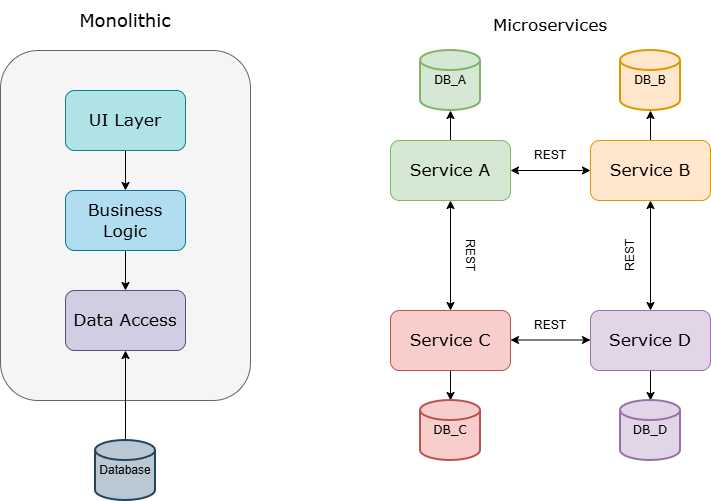
\includegraphics[scale=0.45]{figures/images/chapter2/monolith_vs_microservices.drawio.png}
    \caption{Comparison of monolithic architecture (left) and microservices architecture (right). In the monolithic approach, all modules share a single process and database. In the microservices approach, each service is independently deployable with its own database.}
    \label{fig:monolith-vs-microservices}
\end{figure}

% \textcolor{red}{daca figura e luata de undeva atunci aici in caption pui referinta. Daca iti apartine ca si concept si executie, ignora acest comentariu}

While microservices offer benefits in scalability, team autonomy and technology heterogeneity, they also introduce significant overhead in terms of distributed systems challenges, e.g. network latency, partial failures, data consistency \cite{FowlerMicroservices2014}. When these challenges are poorly managed, they manifest as architectural anti-patterns, i.e. recurring design decisions that negatively impact the quality attributes of the system.

\section{Microservices Anti-Patterns}
\label{sec:anti-patterns}

\par An anti-pattern denotes a frequently used solution to a recurring problem that, rather than resolving it efficiently, introduces a set of negative consequences that may exacerbate the issue further \cite{Brown1998}. In the context of microservices, anti-patterns represent architectural or design decisions that undermine the benefits of the microservices pattern. This section defines and characterizes the anti-patterns targeted by this dissertation, whereas the specific implementation details are presented in Chapter~\ref{chap:ch3}.

\subsection{Shared Database}
\label{subsec:shared-database}

\par The Shared Database anti-pattern occurs when multiple microservices are allowed access to modify the same database schema, which is a violation of the principle of decentralized data management \cite{Richardson2018}. This creates tight coupling between services at the data layer, as changes to the database schema can break multiple services simultaneously. Furthermore, services cannot be independently deployed or scaled without considering the shared database.

As illustrated in Figure~\ref{fig:shared-database}, when services A, B and C all connect to the same database, any schema migration in one service can cause failures in the other. The recommended remediation is to adopt the database-per-service pattern and synchronize data across services using asynchronous events or the Saga pattern \cite{Richardson2018}.

\begin{figure}[htbp]
    \centering
    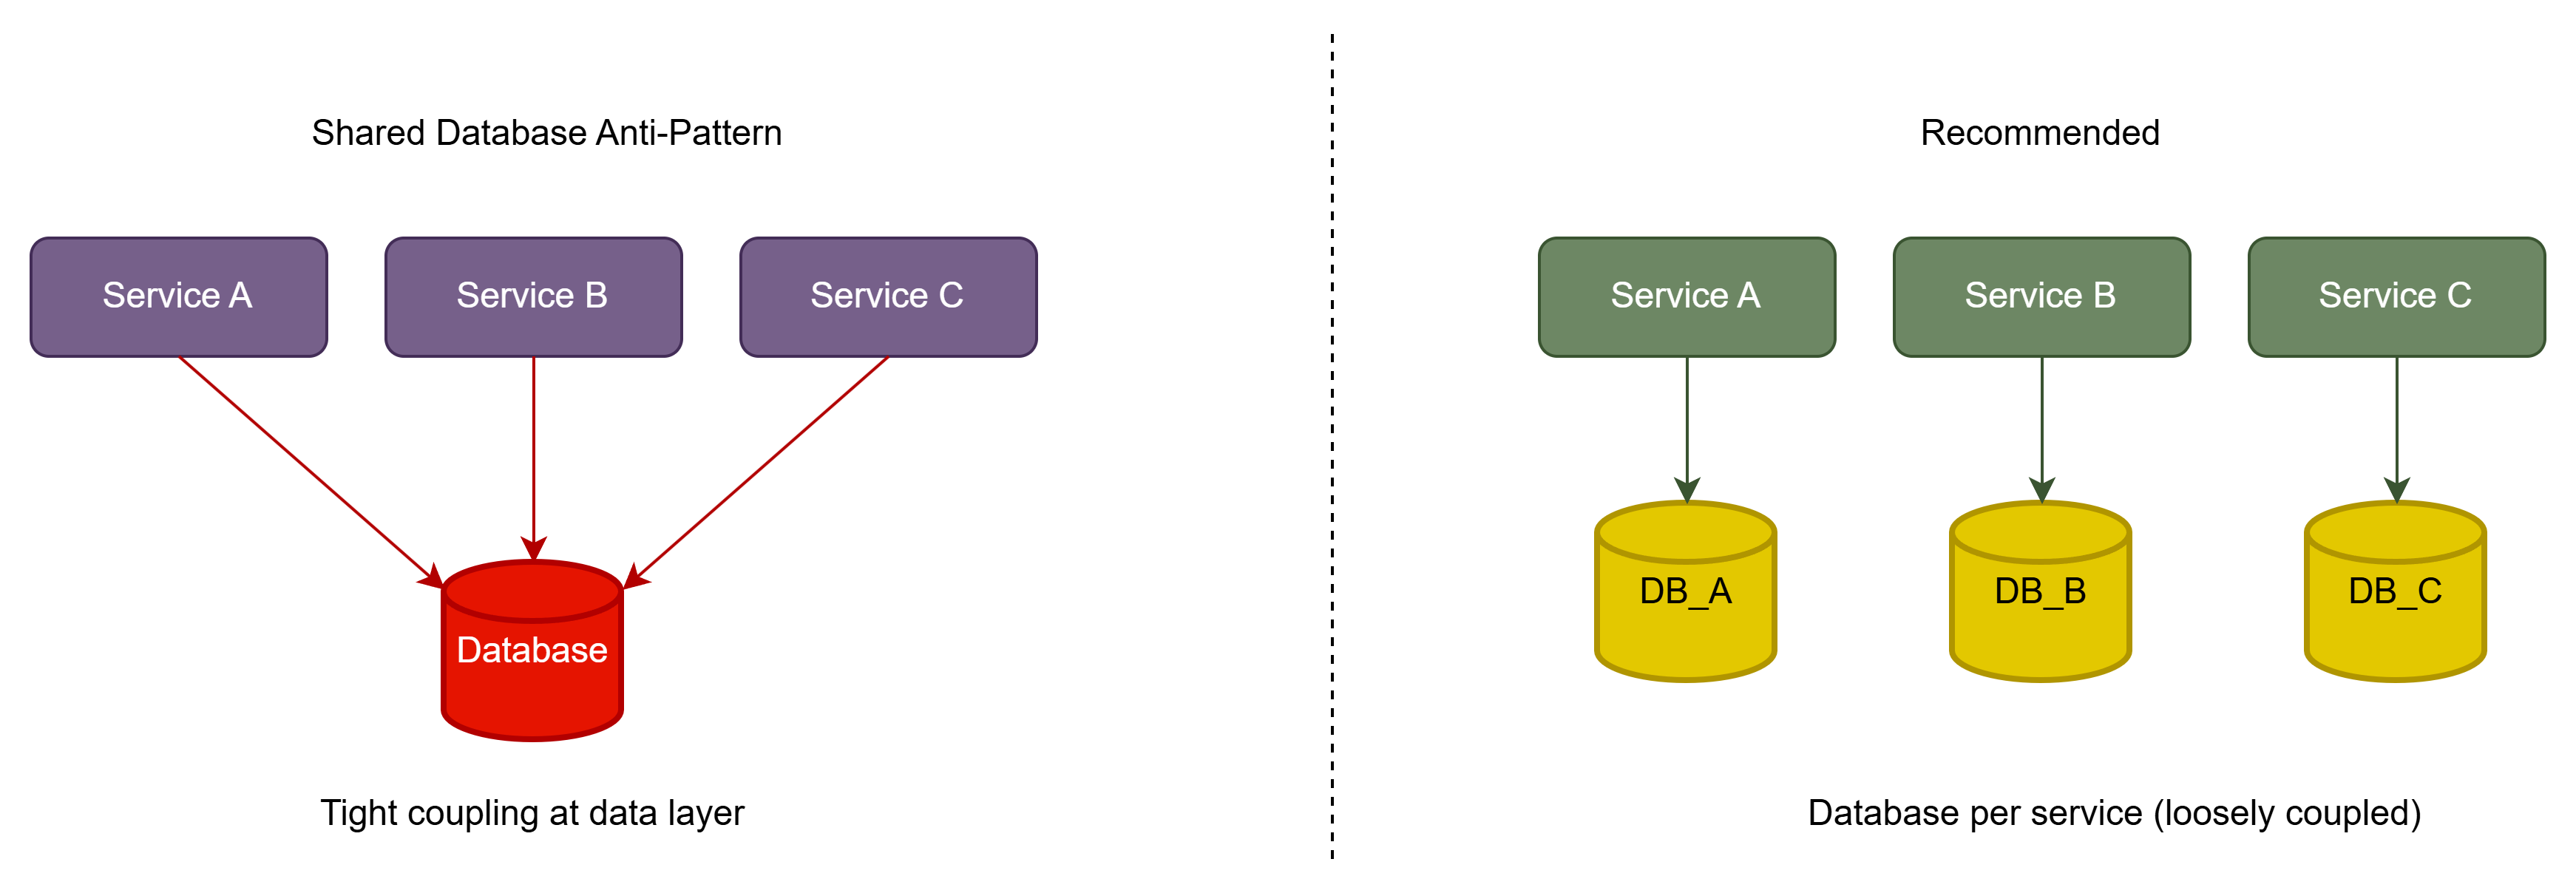
\includegraphics[scale=0.10]{figures/images/chapter2/shared_db.drawio.png}
    \caption{Shared Database Anti-Pattern: multiple services access the same database instance, creating tight coupling at the data layer.}
    \label{fig:shared-database}
\end{figure}

% The concretestatic detection method used for this anti-pattern is presented in Chapter~\ref{chap:ch3}, Section~\ref{subsec:detect-shared-database}.

\subsection{Cyclic Dependency}
\label{subsec:cyclic-dependency}

\par Cyclic dependencies occur when two or more services form a circular chain of dependencies (e.g., in an online shopping application, the Order Service depends on the Payment Service, which depends on the Inventory Service, which in turn depends back on the Order Service, forming a circular dependency). Cycles in the service dependency graph violate the acyclic dependencies principle and create tight coupling, making it fairly difficult to deploy, test, or reason about services independently \cite{Martin2017}.

% The concretegraph-based detection method used for this anti-pattern is presented in Chapter~\ref{chap:ch3}, Section~\ref{subsec:detect-cyclic-dependency}.

Figure~\ref{fig:cyclic-dependency} illustrates a cyclic dependency among three services, as presented in the introduction of this subsection.

\begin{figure}[htbp]
    \centering
    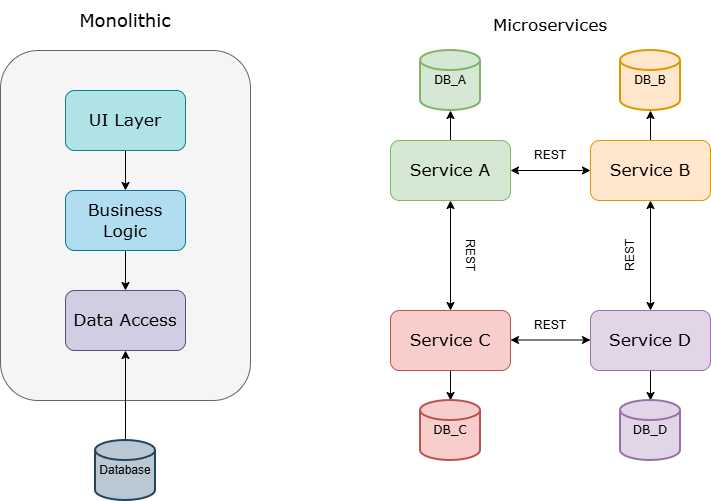
\includegraphics[scale=0.15]{figures/images/chapter2/cyclic-dependency.drawio.png}
    \caption{Example of a cyclic dependency. Services A, B and C form a strongly connected component where no service can be deployed or tested independently.}
    \label{fig:cyclic-dependency}
\end{figure}

\subsection{Nano Service}
\label{subsec:nano-service}

\par A service that is too fine-grained to justify its operational overhead is referred to in this work as a Nano Service, following microservice anti-pattern catalogues that describe nano services as the result of overly fine-grained decomposition \cite{Tighilt2023}. This concern is closely related to the Microservice Greedy smell reported by Taibi and Lenarduzzi, where teams create new microservices even when the resulting services provide very limited functionality \cite{Taibi2018}. Each microservice carries inherent costs: monitoring, deployment pipelines, network communication, and operational maintenance. When a service has very few lines of code and exposes only one or two endpoints, the overhead of running it as an independent process may outweigh the benefits of decomposition.

% The concretethreshold-based detection method used for this anti-pattern is presented in Chapter~\ref{chap:ch3}, Section~\ref{subsec:detect-nano-service}.

The recommended remediation for nano services is to reconsider the service boundary and, when separate deployment is not justified, merge the service with a related, functionally cohesive service \cite{Tighilt2023}.

\subsection{God Service}
\label{subsec:god-service}

\par A God Service is the microservice counterpart of the well-known God Class code smell, also documented as the ''Blob'' anti-pattern \cite{Brown1998}. It refers to a service that handles too many responsibilities, spanning multiple business domains within a single deployable unit. God services grow over time as developers add functionality to an existing service rather than creating new ones, resulting in a service that is difficult to understand, test, and scale independently.

% The concretestructural detection method used for this anti-pattern is presented in Chapter~\ref{chap:ch3}, Section~\ref{subsec:detect-god-service}.

\subsection{Chatty Service}
\label{subsec:chatty-service}

\par The Chatty Service anti-pattern occurs when a service makes an excessive number of fine-grained remote calls to another service to complete a single business operation \cite{Richardson2018}. This increases network latency, reduces throughput, and makes the system fragile to network failures. The chatty communication pattern often indicates that the service boundaries were drawn incorrectly, and data that should be co-located is split across services.

% The concretedetection method used for this anti-pattern is presented in Chapter~\ref{chap:ch3}, Section~\ref{subsec:detect-chatty-service}.

Figure~\ref{fig:chatty-services} contrasts a chatty communication pattern with a well-designed coarse-grained interaction. In the chatty pattern, Service A makes many fine-grained calls to Service B to complete a single operation, whereas the improved design consolidates these into fewer, coarser-grained requests.

\begin{figure}[htbp]
    \centering
    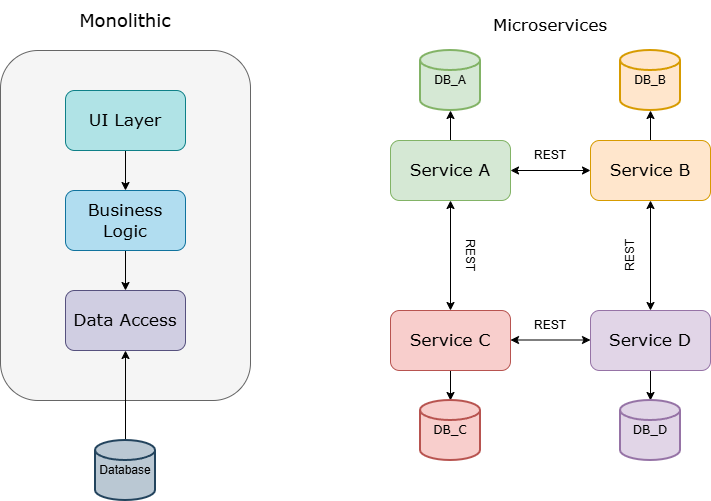
\includegraphics[scale=0.08]{figures/images/chapter2/chatty-services.drawio.png}
    \caption{Example of chatty services versus coarse-grained services. Chatty Service A sends too many requests to Service B, whereas Coarse-Grained Service A sends fewer, more consolidated requests.}
    \label{fig:chatty-services}
\end{figure}

\subsection{Hardcoded Endpoints}
\label{subsec:hardcoded-endpoints}

\par The Hardcoded Endpoints anti-pattern occurs when service URLs are embedded directly in the source code instead of being resolved through a service discovery mechanism (e.g., Netflix Eureka, Consul, or Kubernetes DNS) \cite{Richardson2018}. Hardcoded endpoints create tight coupling between services and make the system inflexible to infrastructure changes such as scaling, failover, or environment migration.

% The concretesource-code detection method used for this anti-pattern is presented in Chapter~\ref{chap:ch3}, Section~\ref{subsec:detect-hardcoded-endpoint}.

\subsection{Distributed Monolith}
\label{subsec:distributed-monolith}

\par The Distributed Monolith anti-pattern describes a system that has been decomposed into multiple services but retains the tight coupling characteristics of a monolithic architecture \cite{Newman2015}. In such a system, services cannot be deployed, tested, or scaled independently, as a change in one service frequently requires coordinated changes and redeployments across several other services. The result is a system that combines the complexity of distributed systems (network latency, partial failures, operational overhead) with none of the benefits of microservices (independent deployability, team autonomy, technology heterogeneity).

A distributed monolith typically arises when services share too many dependencies, communicate excessively, or rely on synchronous call chains to fulfill requests.

% The concretemetric-based detection method used for this anti-pattern is presented in Chapter~\ref{chap:ch3}, Section~\ref{subsec:detect-distributed-monolith}.

The recommended remediation involves identifying and removing unnecessary inter-service dependencies, introducing asynchronous communication where possible, and ensuring that each service encapsulates a well-defined bounded context with minimal external dependencies \cite{Richardson2018}.

\subsection{Additional Anti-Patterns}
\label{subsec:anti-patterns-summary}

\par Beyond the primary anti-patterns described in the preceding subsections, this work targets three additional anti-patterns that address gaps in API governance, service boundary design, and communication topology.

\par API Versioning Absence occurs when services expose REST endpoints without a versioning strategy (e.g.\ a \texttt{/v1/} path prefix), making it harder to introduce breaking API changes while preserving compatibility for existing consumers \cite{Taibi2018, Walker2020}. In rapidly evolving microservice systems, the absence of versioning can force coordinated deployments across consumer services whenever an endpoint's contract changes, undermining the independent deployability that microservices are designed to provide.

% The concretedetection method used for this anti-pattern is presented in Chapter~\ref{chap:ch3}, Section~\ref{subsec:detect-versioning-absence}.

\par Wrong Cuts refers to service boundaries that do not align with business domain boundaries, resulting in high coupling and low cohesion across services \cite{Taibi2018}. When functionality that belongs to a single bounded context is split across multiple services, the resulting inter-service communication overhead and tight coupling negate the benefits of decomposition.

% The concretedetection method used for this anti-pattern is presented in Chapter~\ref{chap:ch3}, Section~\ref{subsec:detect-wrong-cuts}.

\par ESB Misuse occurs when a single service mediates most inter-service communication, effectively recreating the Enterprise Service Bus pattern within a microservices architecture \cite{Richards2015}. This centralisation introduces a single point of failure, a performance bottleneck, and a deployment coupling point that contradicts the decentralised communication principle of microservices.

% The concretedetection method used for this anti-pattern is presented in Chapter~\ref{chap:ch3}, Section~\ref{subsec:detect-esb-misuse}.

Table~\ref{tab:anti-patterns-summary} summarizes all the anti-patterns targeted by this dissertation, along with their severity levels and the Chapter~\ref{chap:ch3} sections that describe their detection methodology.

\begin{table}[!ht]
    \begin{center}
        \begin{tabular}{|l|l|p{180pt}|}
            \hline
            \textbf{Anti-Pattern} & \textbf{Severity} & \textbf{Detection Methodology} \\
            \hline\hline
            Shared Database & High & Section~\ref{subsec:detect-shared-database} \\
            \hline
            Cyclic Dependency & Critical & Section~\ref{subsec:detect-cyclic-dependency} \\
            \hline
            Nano Service & Medium & Section~\ref{subsec:detect-nano-service} \\
            \hline
            God Service & High & Section~\ref{subsec:detect-god-service} \\
            \hline
            Chatty Service & High & Section~\ref{subsec:detect-chatty-service} \\
            \hline
            Hardcoded Endpoints & Medium & Section~\ref{subsec:detect-hardcoded-endpoint} \\
            \hline
            Distributed Monolith & Critical & Section~\ref{subsec:detect-distributed-monolith} \\
            \hline
            API Versioning Absence & Medium & Section~\ref{subsec:detect-versioning-absence} \\
            \hline
            Wrong Cuts & High & Section~\ref{subsec:detect-wrong-cuts} \\
            \hline
            ESB Misuse & High & Section~\ref{subsec:detect-esb-misuse} \\
            \hline
        \end{tabular}
    \end{center}
    \caption{Summary of targeted microservice anti-patterns and references to their detection methodology.}
    \label{tab:anti-patterns-summary}
\end{table}

\section{Related Work}
\label{sec:related-work}

\par The detection of anti-patterns in microservices architectures has received growing attention from the scientific research community. This section reviews the most relevant prior work and positions this dissertation within the existing landscape.

\subsection{Systematic Reviews and Grey Literature Studies}
\label{subsec:systematic-reviews}

\par Several systematic literature reviews have mapped the state of research on microservices, providing a broad understanding of the field's maturity and open challenges.

Di-Francesco et al.\ conducted a systematic mapping study on research related to microservices architecture, analyzing 71 studies published between 2014 and 2016 \cite{DiFrancesco2017}. Their findings revealed that the majority of research focused on migration from monolithic to microservice architectures, with comparatively little attention to quality assurance, anti-pattern detection, and automated analysis tools. The authors identified an appreciable gap between the industrial adoption of microservices and the availability of rigorous academic research that addresses the architectural challenges that practitioners face. This gap motivates the need for tools that can aid development teams in identifying architectural debt in microservice systems.

Soldani et al.\ performed a systematic grey literature review covering 51 industrial experience reports and practitioner blog posts on microservices \cite{Soldani2018}. Their study identified the most frequently reported pains (challenges) and gains (benefits) of microservice adoption. Among the pains, the most commonly reported were increased complexity in distributed systems, difficulties with data management across services, and challenges related to monitoring and debugging. Notably, several of the anti-patterns targeted by this dissertation correspond to the pains reported by the practitioners in the aforementioned study: the Shared Database anti-pattern relates to data management difficulties, the Distributed Monolith corresponds to accidental tight coupling, and the Chatty Service pattern reflects the complexity of managing inter-service communication. The alignment between practitioner-reported challenges and the anti-patterns detected by this work supports its relevance.

\subsection{Empirical Studies on Microservices Anti-Patterns}
\label{subsec:empirical-studies}

\par Taibi and Lenarduzzi conducted an empirical study involving interviews with 72 experienced developers, identifying the most common "bad smells" in microservice architectures \cite{Taibi2018}. Their findings highlighted that Wrong Cuts, Shared Database (also referred to as "Shared Persistency") and Hardcoded Endpoints are among the most frequently encountered and impactful anti-patterns in enterprise practice. The study also reported that many teams were unaware of these anti-patterns until they had accumulated enough significant technical debt, underscoring the value of automated detection tools. This empirical evidence informed the selection of anti-patterns targeted by this dissertation.

In a subsequent work, Taibi, Lenarduzzi, and Pahl proposed a structured taxonomy that catalogues twenty microservice anti-patterns grouped into \emph{technical} and \emph{organizational} categories, each further divided into subcategories, i.e. internal and communication smells on the technical side, and team-oriented and technology/tool-oriented smells on the organizational side \cite{Taibi2020}. This taxonomy provides a principled framework for reasoning about the origins of microservice anti-patterns. Drawing on this and the broader anti-pattern literature, the present dissertation organizes the ten anti-patterns it targets into four architectural dimensions of its own, i.e. service design, communication, data management, and deployment and coupling, as summarized in Table~\ref{tab:antipattern-dimensions}.

\begin{table}[htbp]
    \begin{center}
        \small
        \begin{tabular}{|l|l|p{170pt}|}
            \hline
            \textbf{Architectural Dimension} & \textbf{Anti-Pattern} & \textbf{Concern Addressed} \\
            \hline\hline
            \multirow{2}{*}{Service Design}
            & Nano Service   & Service too small to justify operational overhead \\
            \cline{2-3}
            & God Service    & Service handling too many responsibilities \\
            \hline
            \multirow{4}{*}{Communication}
            & Chatty Service       & Excessive fine-grained inter-service calls \\
            \cline{2-3}
            & Cyclic Dependency    & Circular dependency chains between services \\
            \cline{2-3}
            & ESB Misuse           & Single service mediating most communication \\
            \cline{2-3}
            & Hardcoded Endpoints  & Service URLs hardcoded instead of using discovery \\
            \hline
            Data Management
            & Shared Database      & Multiple services accessing the same database \\
            \hline
            \multirow{3}{*}{Deployment \& Coupling}
            & Distributed Monolith    & Tightly coupled services requiring co-deployment \\
            \cline{2-3}
            & Wrong Cuts              & Misplaced service boundaries causing high coupling \\
            \cline{2-3}
            & API Versioning Absence  & No API versioning strategy detected \\
            \hline
        \end{tabular}
    \end{center}
    \caption{Mapping of the ten anti-patterns detected by this work to four architectural dimensions. The grouping is the author's own, inspired by the microservice anti-pattern literature \cite{Taibi2018, Taibi2020}.}
    \label{tab:antipattern-dimensions}
\end{table}

Bogner et al.\ conducted a literature review investigating maintainability measurement for service- and microservice-based systems \cite{Bogner2019}. They mapped candidate metrics to four dominant design properties, i.e.\ size, complexity, coupling and cohesion, and argued that microservice-specific factors such as many services, technological heterogeneity and decentralised control make automatic metric collection difficult without specialised tool support. This observation aligns with a notable contribution of this dissertation: combining intra-service code smell detection with inter-service dependency analysis to provide a panoramic assessment of architectural quality.

\subsection{Static Analysis Approaches}
\label{subsec:related-static}

\par Neri et al.\ conducted a multivocal review of microservice design principles and the architectural smells that violate them \cite{Neri2020}. Their work catalogued seven architectural smells, framed as violations of design principles such as service autonomy, decentralized data management, and smart endpoints and dumb pipes, together with sixteen refactorings to resolve them. While their work provides a strong principled foundation for reasoning about microservice quality, it does not integrate code-level smell detection into the architectural analysis and does not provide an implemented tool with configurable thresholds.

Sharma and Spinellis provided a comprehensive survey on software smells and demonstrated the role of automated tools in detecting them \cite{Sharma2018}. DesigniteJava, presented as a large-scale multi-faceted code smell detection tool by Sharma \cite{Sharma2024}, detects code smells and computes object-oriented metrics for Java projects. While DesigniteJava operates at code level within individual projects, this dissertation uses the aggregate density of these smells as the code-quality signal that contributes to the composite health score, complementing the architectural-level analysis carried out through Spoon-based structural metrics and dependency-graph algorithms.

Pigazzini et al.\ proposed an approach for detecting microservice smells by combining structural analysis with dependency extraction \cite{Pigazzini2020}. Their work focused on identifying smells such as Cyclic Dependencies, Hardcoded Endpoints, and Shared Persistence by analyzing dependency structure extracted from Docker and Spring configuration files (\texttt{docker-compose.yml}, \texttt{Dockerfile}, \texttt{application.yml}) together with source-code communication patterns such as Feign and \texttt{RestTemplate} usage. While their approach addresses inter-service structural smells, it does not incorporate intra-service code smell analysis and does not support the breadth of anti-patterns covered by this dissertation.

Cerny et al.\ provided a contextual analysis of microservice architecture, surveying current research directions and identifying gaps in automated analysis capabilities \cite{Cerny2018}. They highlighted the need for tools that can automatically reconstruct microservice architectures from source code and detect anti-patterns without requiring manual configuration. The automated microservice detection mechanism implemented in this work directly addresses this need by scanning for build files and applying a deployability gate to identify service boundaries without manual configuration.

\subsection{Dynamic and Hybrid Approaches}
\label{subsec:related-dynamic}

\par Dynamic analysis approaches monitor running systems to detect anti-patterns from runtime behaviour. Distributed tracing tools such as Jaeger or Zipkin can reveal chatty communication patterns and cyclic call chains at runtime by recording the flow of requests across service boundaries. However, dynamic approaches require a running system with representative workloads and instrumented services, making them less suitable for early-stage analysis, code review workflows, or integration into CI/CD pipelines where the system is not deployed.

Hybrid approaches combine static and dynamic analysis. For instance, a tool might perform static dependency extraction from source code and complement it with runtime call frequency data collected via distributed tracing. While hybrid approaches can provide higher accuracy (e.g. by confirming the a statically detected dependency is actually exercised at runtime), they introduce additional complexity and infrastructure requirements. They also require the system to be deployed and exercised with representative traffic, which is not always feasible.

This dissertation focuses on static analysis to enable anti-pattern detection without requiring a running system, making it applicable to source repositories at any stage of development. This design choice prioritizes broad applicability and ease of integration over the higher precision that runtime data could provide.

\subsection{Automated Detection Tools}
\label{subsec:related-tools}

\par Several tools have been developed for microservice analysis. This subsection reviews the most relevant ones and highlights their strengths and limitations relative to this work.

\par Arcan serves as a tool developed for detection and analysis of architectural smells in Java projects that supports dependency graph analysis and cycle detection \cite{Arcelli2017}. It detects architectural smells such as Cyclic Dependencies and Unstable Dependencies by constructing and analyzing a dependency graph from compiled Java bytecode. However, Arcan was primarily designed with monolithic Java applications in mind and does not specifically target microservice anti-patterns such as Shared Database (or Persistence), Chatty Service or Distributed Monolith. It also does not provide automated microservice boundary detection or a composite health score.

\par MicroART recovers the architecture of microservice-based systems by combining static information from the source repository with dynamic analysis of the running system \cite{Granchelli2017}. It clones the project's repository to extract service metadata and then monitors the deployed containers at runtime, querying the Docker runtime and capturing inter-service network traffic to reconstruct the actual service interactions, which an architect can subsequently refine. While MicroART does address the important problem of architecture recovery, it focuses on visualization rather than anti-pattern detection. It does not analyze source code for code smells, does not compute coupling metrics and does not provide remediation recommendations.

\par MSANose is a detection tool specifically designed for microservice smells, based on the catalog established by Taibi et al.\ \cite{Walker2020}. It detects smells such as Shared Database, Cyclic Dependencies, Hardcoded Endpoints, ESB Usage, Wrong Cuts, API Versioning, and Microservice Greedy through static analysis for Java-based microservice projects. MSANose represents one close prior work to this dissertation, particularly among static Java-based microservice smell detectors. However, it differs in several respects: it does not integrate a general intra-service code-level smell catalogue into the architectural assessment, it does not compute a composite health score, and it does not target God Service or Chatty Service as defined and implemented in this dissertation.

\par MARS, proposed by Tighilt et al., is a tool-supported approach for specifying and detecting microservice anti-patterns through source-code analysis \cite{Tighilt2023}. It targets sixteen microservice anti-patterns and was empirically validated on 24 microservice-based systems, reporting an average precision of 82\% and recall of 89\%. MARS therefore provides broader anti-pattern coverage than this dissertation. The contribution of the present work is positioned differently: it focuses on a selected set of ten anti-patterns and combines their detection with DesigniteJava-based intra-service smell density, Spoon-based structural metrics, a composite architectural health score, evidence snippets, remediation guidance, analysis history, and a web/API workflow for Java Spring Boot projects.

% Table~\ref{tab:related-tools-comparison} provides a detailed feature comparison of these tools against the system presented in this dissertation.
%
% \begin{table}[htbp]
%     \begin{center}
%         \small
%         \begin{tabular}{|p{100pt}|c|c|c|c|}
%             \hline
%             \textbf{Feature} & \textbf{Arcan} & \textbf{MicroART} & \textbf{MSANose} & \textbf{This Work} \\
%             \hline\hline
%             Targets microservices & $\times$ & \checkmark & \checkmark & \checkmark \\
%             \hline
%             General intra-service code smell detection & \checkmark & $\times$ & Partial & \checkmark \\
%             \hline
%             Cycle detection & \checkmark & $\times$ & \checkmark & \checkmark \\
%             \hline
%             Shared database detection & $\times$ & $\times$ & \checkmark & \checkmark \\
%             \hline
%             God service detection & $\times$ & $\times$ & $\times$ & \checkmark \\
%             \hline
%             Chatty service detection & $\times$ & $\times$ & $\times$ & \checkmark \\
%             \hline
%             Hardcoded endpoints & $\times$ & $\times$ & \checkmark & \checkmark \\
%             \hline
%             ESB misuse detection & $\times$ & $\times$ & \checkmark & \checkmark \\
%             \hline
%             Wrong cuts detection & $\times$ & $\times$ & \checkmark & \checkmark \\
%             \hline
%             API versioning check & $\times$ & $\times$ & \checkmark & \checkmark \\
%             \hline
%             Auto service discovery & $\times$ & Partial & $\times$ & \checkmark \\
%             \hline
%             Health score metric & $\times$ & $\times$ & $\times$ & \checkmark \\
%             \hline
%             Web interface / API & $\times$ & \checkmark & $\times$ & \checkmark \\
%             \hline
%             Configurable thresholds & $\times$ & $\times$ & Partial & \checkmark \\
%             \hline
%             Code snippet evidence & $\times$ & $\times$ & $\times$ & \checkmark \\
%             \hline
%             Remediation guidance & $\times$ & $\times$ & $\times$ & \checkmark \\
%             \hline
%             Target language & Java & Multi & Java & Java \\
%             \hline
%             Analysis technique & Static & Hybrid & Static & Static \\
%             \hline
%         \end{tabular}
%     \end{center}
%     \caption{Feature comparison of related architectural analysis tools. \checkmark\ indicates the feature is supported, $\times$\ indicates it is not supported. ''Partial'' indicates limited support. For MSANose, ''Partial'' in the intra-service code-smell row means it detects microservice-specific smells but does not integrate a general intra-service smell catalogue such as DesigniteJava or use smell density as a health-score dimension; ''Partial'' in the configurable-thresholds row reflects that it exposes only a single adjustable ESB connectivity threshold rather than broadly externalized configuration.}
%     \label{tab:related-tools-comparison}
% \end{table}

\subsection{Positioning and Contributions of This Work}
\label{subsec:positioning}

\par This dissertation differentiates itself from existing work in several ways, addressing gaps identified in the reviewed literature.

First, this work performs multi-level analysis. Existing tools typically operate at a single level of abstraction: either code-level smell detection (e.g.\ DesigniteJava) or architectural-level dependency analysis (e.g.\ Arcan, MicroART). This work combines intra-service code analysis, comprising DesigniteJava smell density together with Spoon-based structural metrics, with inter-service architectural analysis via graph algorithms, providing a more comprehensive assessment. For example, code-level structural metrics such as class cohesion, computed via Spoon, are used as evidence for flagging god services at the architectural level.

Second, the tool offers coverage across several architectural dimensions, detecting ten selected anti-patterns: service design (Nano Service, God Service), inter-service communication (Chatty Service, Cyclic Dependency, Hardcoded Endpoints, ESB misuse), data management (Shared Database), and system-level coupling (Distributed Monolith, API Versioning Absence, Wrong Cuts). Although MARS covers a larger catalogue of anti-patterns, this work emphasizes the integration of selected service-level and system-level findings with code-level smell evidence, configurable thresholds, evidence snippets, remediation guidance, and a composite health score.

Third, the tool provides automated microservice detection by automatically identifying microservice boundaries within a multi-module project. Candidate modules are first discovered by scanning for build files (\texttt{pom.xml}, \texttt{build.gradle}, \texttt{build.gradle.kts}) and are then filtered through a \textit{deployability gate} that verifies whether each candidate is an independently deployable service using three signals applied in priority order: a framework entry point (e.g.\ \texttt{@SpringBootApplication}), the presence of a Dockerfile, or a \texttt{main()} method. This eliminates the need for manual service enumeration, which is required by most existing tools. Multi-module Maven and Gradle projects are supported, with automatic filtering of non-service modules (e.g.\ examples, tests, build support) and parent aggregator modules.

Fourth, detection thresholds for metrics-based anti-patterns are externalized as configurable detection parameters (via Spring Boot's \texttt{application.yml}), allowing calibration to project-specific norms. For instance, the LOC threshold for nano service detection or the call count threshold for chatty service detection can be adjusted without modifying the source code.

Fifth, a composite health score provides a single numeric metric (0-100) for architectural quality, accompanied by a letter grade (A through F). Unlike a simple aggregate, the score is decomposed into four weighted categories, anti-pattern severity, code quality, architectural coupling, and service sizing, each with an itemized list of deductions. Because each deduction is attributed to a specific finding within one of these categories, a low score can be traced back to the dimension that caused it rather than read as a single opaque number, and the per-category scores can be compared across successive analysis runs.

Sixth, unlike existing tools that report anti-patterns as abstract findings, this work supports evidence-based reporting with code snippets attached to each detected anti-pattern. When a cyclic dependency is detected, the tool extracts and presents the relevant \texttt{@FeignClient} annotation or \texttt{RestTemplate} invocation from the source code, providing developers with immediate context for understanding and remediating the issue.

Finally, the tool is delivered as a web application with a RESTful API, supporting both interactive use through a web dashboard and programmatic integration into CI/CD pipelines for continuous architectural quality monitoring. Users can submit projects for analysis either by uploading a ZIP archive or by providing a Git repository URL, which is cloned automatically via JGit.

\section{Summary}
\label{sec:summary}

\par This chapter has established the theoretical and related-work foundation for this dissertation. The microservices architectural style was introduced along its core principles, inherent challenges and a taxonomy of ten microservice anti-patterns.

The related work was reviewed across four categories: systematic literature reviews that map the research landscape, empirical studies that identify practitioner-reported anti-patterns, static analysis approaches that formalize detection techniques, and automated tools that implement detection. The review revealed that existing tools tend to operate at a single level of abstraction or focus on particular subsets of architectural concerns. This dissertation addresses these gaps by combining intra-service and inter-service analysis, supporting ten anti-patterns across four architectural dimensions, providing automated microservice detection, configurable thresholds, evidence-based reporting with code snippets, and a category-based composite health score with letter grading for tracking architectural quality over time. The next chapter presents the detailed detection methodology for each anti-pattern.

\chapter{Detection Methodology}
\label{chap:ch3}

\par This chapter presents the detection methodology employed by the system developed in this dissertation. It begins with an overview of the analysis pipeline and the foundational techniques, i.e. static code analysis, AST-based source code inspection and code smell detection, then describes the construction and analysis of the interservice dependency graph and the composite health score computation. The chapter concludes with a detailed description algorithm for each individual anti-pattern.

\section{Detection Techniques}
\label{sec:detection-techniques}

\par This section outlines the techniques used for detecting architectural anti-patterns in microservice systems. Figure~\ref{fig:analysis-pipeline} provides an overview of the analysis pipeline, showing how source code is processed through multiple stages to produce anti-pattern detection results.

\begin{figure}
    \centering
    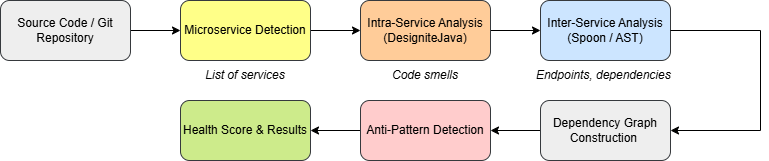
\includegraphics[scale=0.45]{figures/images/chapter3/analysis_pipeline.drawio.png}
    \caption{Overview of the anti-pattern detection pipeline. Source code is processed through microservice detection, intra-service and inter-service analysis, dependency graph construction, and anti-pattern detection, producing a health score and detailed results.}
    \label{fig:analysis-pipeline}
\end{figure}

\subsection{Static Code Analysis}
\label{subsec:static-analysis}

\par Static code analysis examines source code without executing it, allowing detection of structural issues, code smells, and architectural violations at the source level \cite{Chess2007}. In the context of microservices, static analysis can be applied at two levels. Intra-service analysis examines the internal structure of each microservice for code-level smells such as God Class, Long Method, Feature Envy, and Complex Method. The aforementioned smells serve as indicators of architectural problems at the service level. Inter-service analysis, on the other hand, examines the communication patterns, dependencies, and shared resources across microservices to detect architectural anti-patterns such as cyclic dependencies and shared databases.

\subsection{Abstract Syntax Tree Analysis with Spoon}
\label{subsec:spoon-analysis}

\par Spoon is an open-source library for analyzing, transforming and generating Java source code \cite{Pawlak2016}. It builds a fine-grained Abstract Syntax Tree (AST) that provides full access to all elements of the Java programming language, including annotations, method invocations and type references.

In this work, Spoon is used for inter-service analysis, specifically in three ways. Firstly, it detects REST controller endpoints by scanning for \texttt{@RestController}, \texttt{@GetMapping}, \texttt{@PostMapping} and other related annotations. Furthermore, it is used to identify inter-service communication by analyzing \texttt{@FeignClient} annotations, \texttt{@RestTemplate} method calls, and \texttt{@WebClient} builder patterns. Lastly, it extracts service metadata such as the number of endpoints, controller classes and API versioning information.

Beyond inter-service analysis, Spoon is also used for intra-service structural analysis. The God Service detector (Section~\ref{subsec:detect-god-service}) computes per-class metrics such as field count, public method count, import domain count, constructor parameter count and Tight Class Cohesion (TCC) directly from the AST. Similarly, the Chatty Service detector (Section~\ref{subsec:detect-chatty-service}) scans for interfaces and classes that exhibit chatty HTTP~client patterns by inspecting method annotations and verifying invocation target types.

The AST-based approach is more robust than regular expression-based scanning, as it understands the syntactic structure of the code and can resolve annotation attributes, method call chains and type hierarchies.

\subsection{Code Smell Detection with DesigniteJava}
\label{subsec:designite-analysis}

\par DesigniteJava is a static analysis tool that detects design smells, implementation smells and architecture smells in Java projects \cite{Sharma2018}. It analyzes Java source code and produces CSV reports categorizing detected smells by type, affected class and file location.

% The tool detects three categories of smells, summarized in Table~\ref{tab:code-smell-categories}.

In this dissertation, DesigniteJava is integrated as an external tool invoked as a subprocess. The analysis pipeline passes each detected microservice's source directory to DesigniteJava, parses the resulting CSV output files (\texttt{DesignSmells.csv}, \texttt{ImplementationSmells.csv}, \texttt{ArchitectureSmells.csv}), and stores the results in the application database. The God Class smell frequency per service is then used as a signal for god service detection (see Section~\ref{subsec:god-service}).

\begin{table}[htbp]
    \centering
    \footnotesize
    \begin{tabular}{|l|l|p{5.5cm}|l|}
        \hline
        \textbf{Category} & \textbf{Smell Name} & \textbf{Description} & \textbf{Severity} \\
        \hline\hline
        \multirow{4}{*}{Design} & God Class & Class with too many responsibilities & High \\
        \cline{2-4}
        & Feature Envy & Method more interested in other classes & High \\
        \cline{2-4}
        & Insufficient Modularization & Large, poorly modularized class & Medium \\
        \cline{2-4}
        & Unnecessary Abstraction & Abstraction without clear purpose & Low \\
        \hline
        \multirow{4}{*}{Implementation} & Long Method & Method with excessive length & Medium \\
        \cline{2-4}
        & Complex Method & Method with high cyclomatic complexity & Medium \\
        \cline{2-4}
        & Long Parameter List & Method with too many parameters & Medium \\
        \cline{2-4}
        & Magic Number & Unexplained numeric literals & Low \\
        \hline
        \multirow{3}{*}{Architecture} & Cyclic Dependency & Circular dependencies between packages & High \\
        \cline{2-4}
        & Unstable Dependency & Depending on less stable components & Medium \\
        \cline{2-4}
        & Hub-like Dependency & Class depended upon by many others & Medium \\
        \hline
    \end{tabular}
    \caption{Code smell categories detected by DesigniteJava, with their descriptions and severity mappings used in this work.}
    \label{tab:code-smell-categories}
\end{table}

\subsection{Dependency Graph Construction and Analysis}
\label{subsec:graph-analysis}

\par The dependency graph is a directed graph $G = (V, E)$ where each vertex $v \in V$ represents a microservice and each edge $e = (s, t) \in E$ represents a dependency from service $s$ to service $t$. Edges are annotated with metadata including the dependency type (REST synchronous, Feign client, messaging, etc.) and the call count.

\par A central challenge in dependency graph construction is resolving the target of an inter-service call to an actual microservice in the project. In real-world codebases, services are referenced by a variety of identifiers: directory names, \texttt{spring\-.application.name} values, \texttt{localhost:PORT} URLs, or Spring property placeholders injected via \texttt{@Value} annotations. To address this, the dependency graph builder employs a multi-strategy resolution pipeline.

\par The first step is a configuration pre-scan: before scanning source code, each service's \texttt{application.yml} or \texttt{application.properties} is parsed. The \texttt{spring\-.application.name} property is registered as an alias for the service directory name, and \texttt{server.port} values are recorded in a port-to-service mapping. Next, the pipeline performs \texttt{@Value} field resolution, in which fields annotated with Spring's \texttt{@Value} (e.g., \texttt{@Value("\$\{order\--service.url:http://localhost:8081\}")}) are pre-scanned using Spoon. Property placeholders are resolved against the service's configuration, falling back to default values when the property key is not found. Finally, a cascading target resolution strategy is applied: when a call target is extracted from a \texttt{@FeignClient} annotation, \texttt{RestTemplate} invocation, or \texttt{WebClient} call, it is matched to a microservice using three strategies applied in order, i.e. exact match against service names and registered aliases, port-based matching for \texttt{localhost:PORT}-style targets, and fuzzy substring matching with common suffix stripping (e.g., matching ''order'' to ''order-service''). For \texttt{@FeignClient} interfaces, each non-default, non-static method is registered as a separate call evidence entry, since each method corresponds to an individual HTTP request at runtime. This produces accurate per-method call counts that feed into chatty service detection.

Figure~\ref{fig:dependency-graph-example} shows an example dependency graph for a hypothetical microservice system. Each node represents a service, and edges are labeled with the dependency type and call count. The graph reveals a cycle between the Order, Inventory and Payment services as well as a potential ESB misuse pattern where the API Gateway mediates most communication.

\begin{figure}
    \centering
    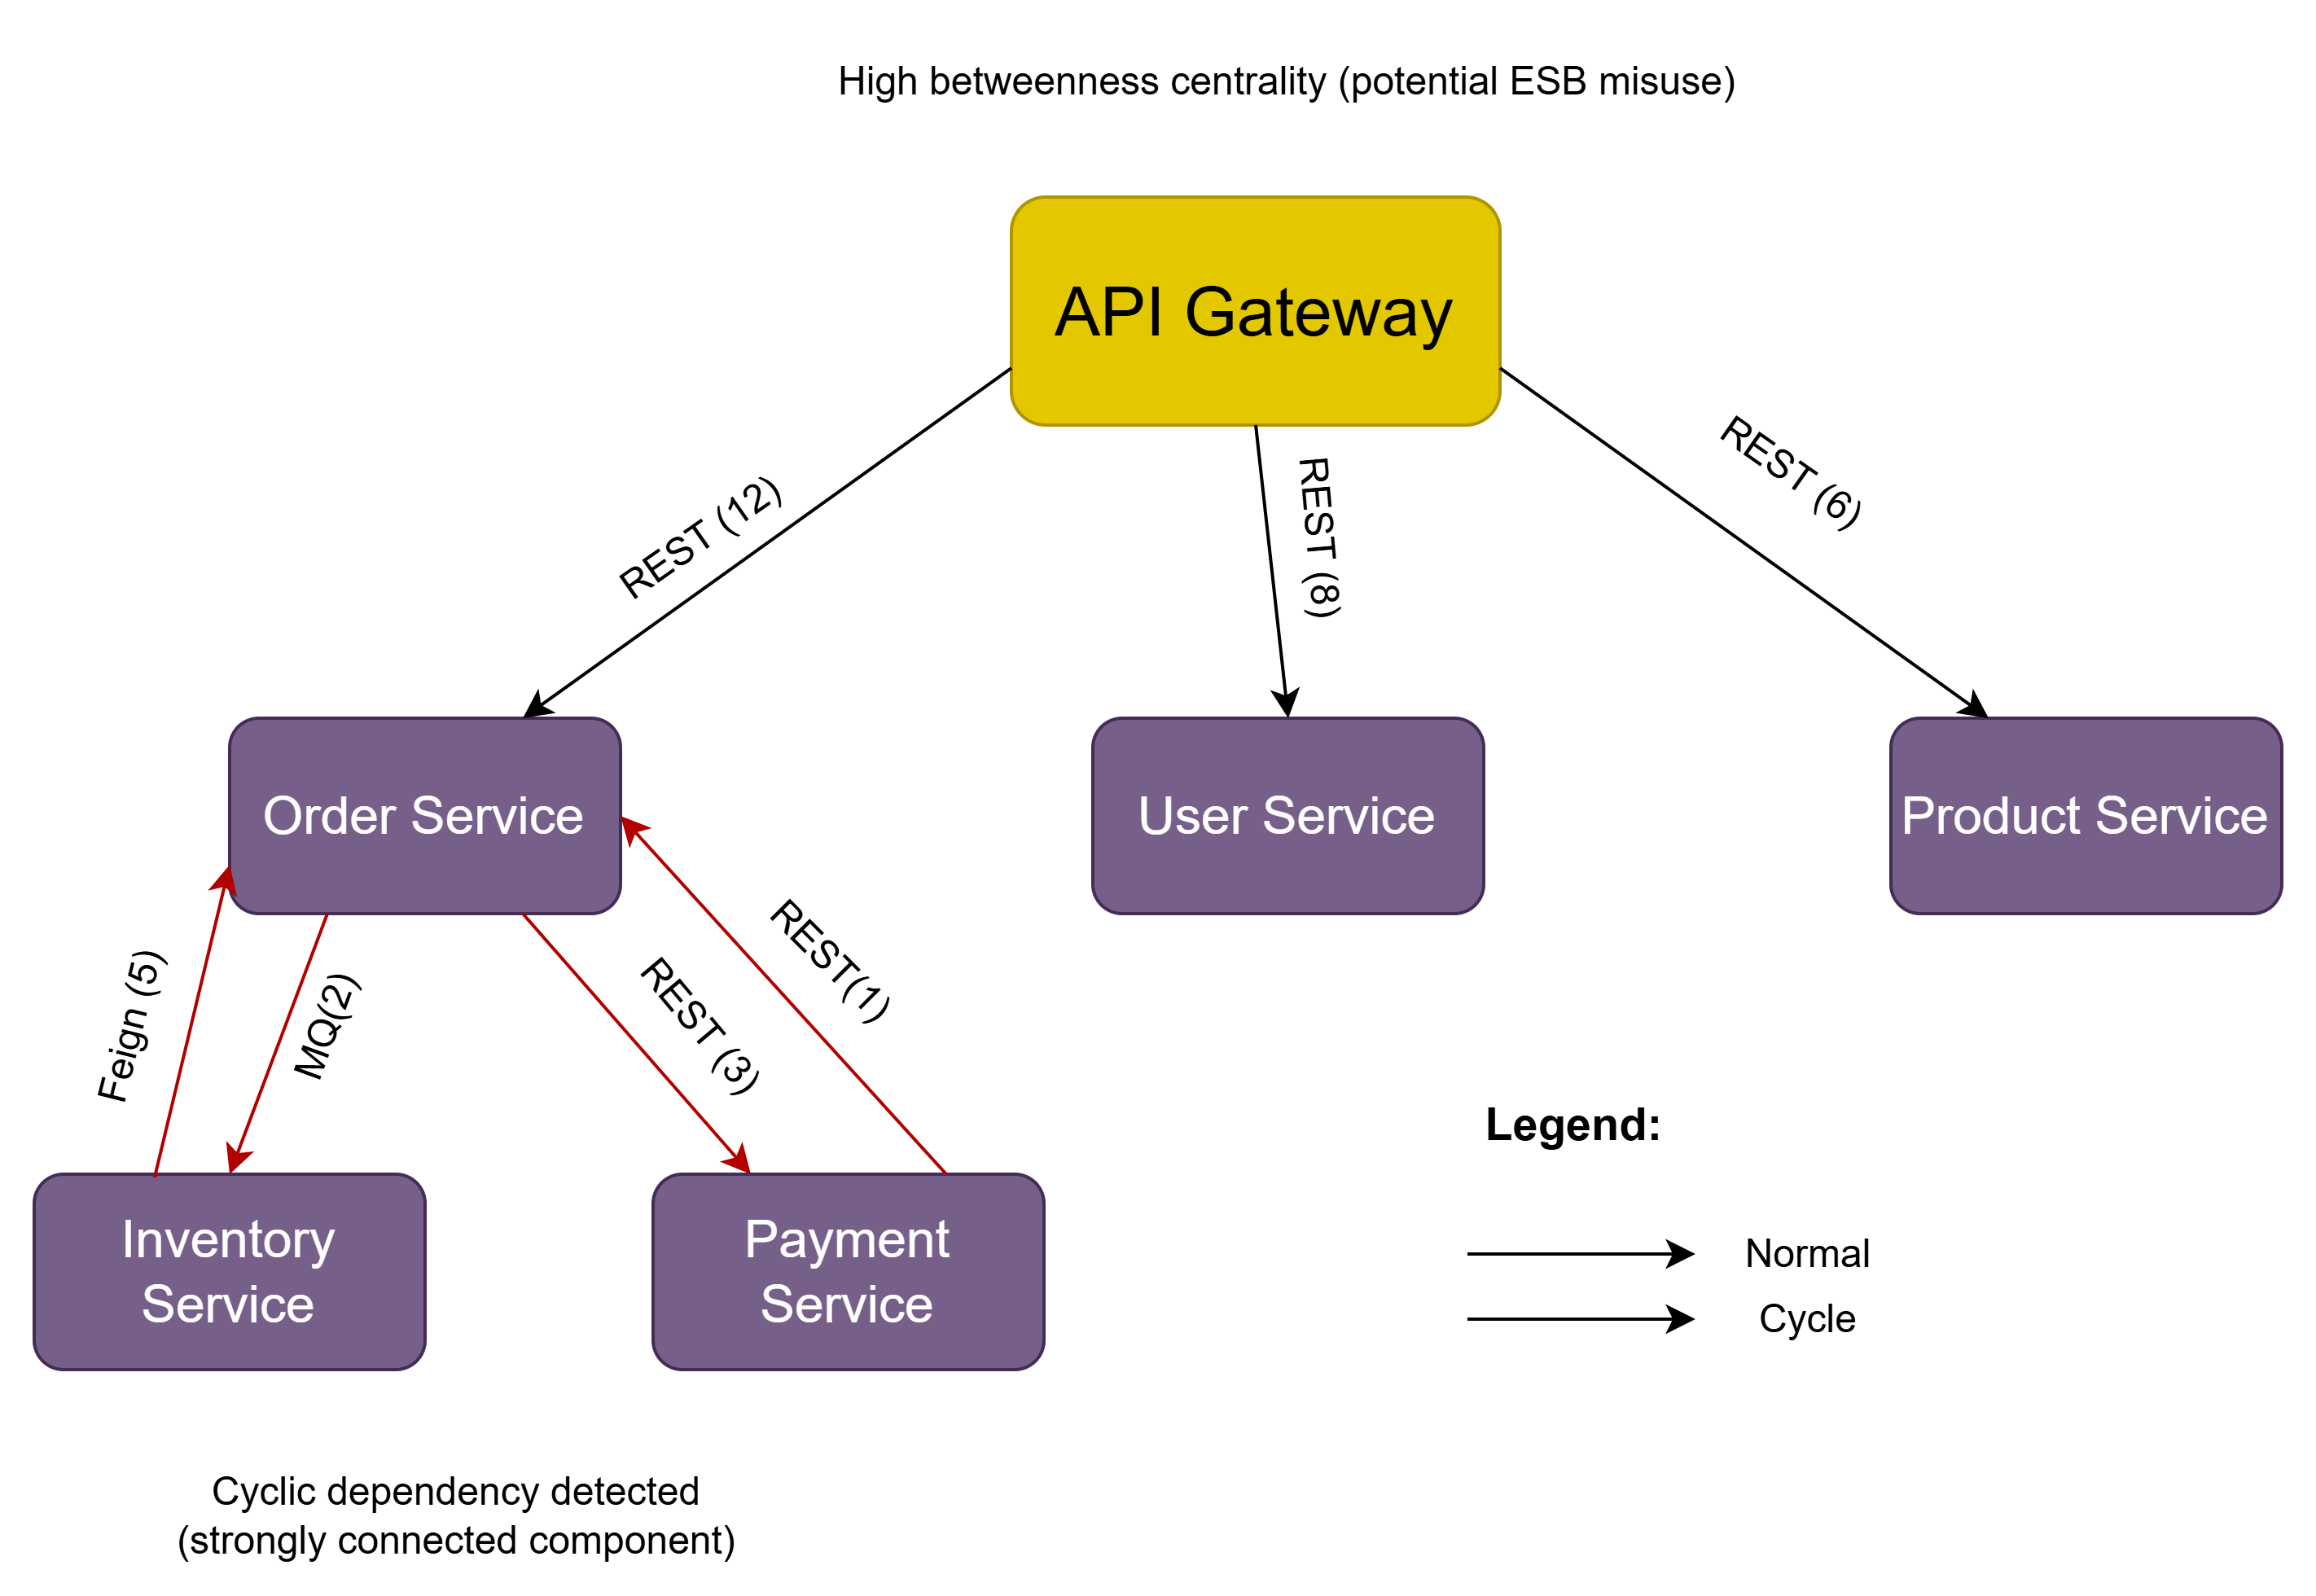
\includegraphics[scale=0.1]{figures/images/chapter3/dependency_graph_example.png}
    \caption{Example dependency graph for a microservice system. Nodes represent services, edges represent dependencies with type and call count annotations. The red dashed edges indicate a cyclic dependency. The API Gateway node exhibits high centrality, potentially indicating ESB misuse.}
    \label{fig:dependency-graph-example}
\end{figure}

\par Graph-based anti-pattern detection encompasses several analytical techniques. Cycle detection involves finding strongly connected components using Tarjan's algorithm to identify cyclic dependencies, while centrality analysis computes betweenness centrality to detect potential ESB misuse, where a single service mediates a disproportionate share of communication. Additionally, coupling metrics are evaluated by computing the coupling coefficient as the ratio of actual dependencies to possible dependencies.

\begin{equation}
    C = \frac{|E|}{|V| \times (|V| - 1)}
    \label{eq:coupling-coefficient}
\end{equation}

\noindent A high coupling coefficient suggests that the system may be a distributed monolith rather than a collection of loosely coupled services.

\subsection{Health Score Computation}
\label{subsec:health-score}

% TO-DO: go into a bit more depth maybe and/or revise this score

\par To provide an overall assessment of a system's architectural health, this dissertation computes a composite health score using a category-based decomposition. The total budget of 100~points is divided across four categories, each with an independent cap:

\begin{equation}
    H = S_{\mathrm{ap}} + S_{\mathrm{cq}} + S_{\mathrm{arch}} + S_{\mathrm{sz}}
    \label{eq:health-score}
\end{equation}

\noindent where each category score $S_i = \max(0,\; M_i - P_i)$, with $M_i$ the maximum budget and $P_i$ the total penalty for that category. The four categories and their budgets are described in the following paragraphs.

\par The first category, Anti-Patterns ($M_{\mathrm{ap}} = 40$), penalises each detected anti-pattern according to its severity (Table~\ref{tab:severity-weights}). The deduction per issue is 8~points for critical severity, 5 for high, 3 for medium, and 1 for low.

\par The second category, Code Quality ($M_{\mathrm{cq}} = 20$), captures the density of code smells reported by DesigniteJava. The penalty is computed on a logarithmic scale, $P_{\mathrm{cq}} = \min(20,\; \lfloor \ln(1 + n_{\mathrm{smells}}) \times 3.5 \rceil)$, which dampens the impact of very large smell counts while still penalising smell-heavy codebases.

\par The third category, Architecture ($M_{\mathrm{arch}} = 25$), assesses the structural quality of the dependency graph. The penalty is derived from the coupling coefficient, $\min(15,\; \lfloor c \times 15 \rceil)$ when $c > 0.1$, and the number of dependency cycles, $\min(10,\; 5 \times n_{\mathrm{cycles}})$.

\par The fourth category, Service Sizing ($M_{\mathrm{sz}} = 15$), evaluates the appropriateness of individual service granularity. Nano services incur a penalty of 3~points each (capped at~8) and god services incur 5~points each (capped at~10).


\par The final score is clamped to $[0, 100]$ and mapped to a letter grade: A~($\geq 90$), B~($\geq 80$), C~($\geq 65$), D~($\geq 50$), F~($< 50$). This category-based decomposition enables teams to identify which quality dimension contributes most to architectural debt and to track improvements per category over time.

Table~\ref{tab:severity-weights} details the severity levels, their corresponding penalty weights in the anti-pattern category, and examples of anti-patterns assigned to each level.

\begin{table}[htbp]
    \centering
    \footnotesize
    \begin{tabular}{|l|c|c|p{6.5cm}|}
        \hline
        \textbf{Severity} & \textbf{Weight} & \textbf{Penalty} & \textbf{Example Anti-Patterns} \\
        \hline\hline
        Critical & 4 & $-8$ per issue & Cyclic Dependency, Distributed Monolith \\
        \hline
        High & 3 & $-5$ per issue & Shared Database, God Service, Wrong Cuts, Chatty Service, ESB Misuse \\
        \hline
        Medium & 2 & $-3$ per issue & Nano Service, Hardcoded Endpoints, API Versioning Absence \\
        \hline
        Low & 1 & $-1$ per issue & --- \\
        \hline
    \end{tabular}
    \caption{Severity levels with their penalty deductions in the anti-pattern category of the health score computation (Equation~\ref{eq:health-score}).}
    \label{tab:severity-weights}
\end{table}

\section{Per-Anti-Pattern Detection Methodology}
\label{sec:per-anti-pattern-detection}

\par This section describes the detection algorithm for each anti-pattern targeted by this work. For each anti-pattern, the input data, detection logic, configurable thresholds, and evidence collection mechanism are presented. The definitions and motivations for each anti-pattern were introduced in Chapter~\ref{chap:ch2}; this section focuses on the \textit{how} of detection.

\subsection{Shared Database Detection}
\label{subsec:detect-shared-database}

\par The Shared Database detector operates by comparing the datasource connection URLs configured across all detected microservices. The algorithm proceeds in two phases.

In the first phase, the configuration files of each microservice are parsed to extract the datasource URL. For Spring Boot applications, the detector reads \texttt{application.yml}, \texttt{application.yaml}, or \texttt{application.properties} configuration files located in the \texttt{/resources} directory of each service. From YAML files, the nested property \texttt{spring.datasource.url} is extract using a recursive map traversal, whereas from properties files, the same key is read directly. Spring property placeholders with default values (e.g., \texttt{\$\{DB\_HOST:localhost\}}) are resolved to their defaults to enable meaningful comparison.

In the second phase, microservices are grouped by their resolved datasource URL. Any group containing more than one service indicates a shared database instance. Formally, let $\mathcal{S}$ denote the set of all microservices and $\mathit{dsUrl}$ denote the resolved datasource URL of service $s$. The detector reports a Shared Database anti-pattern for each equivalence class:

\begin{equation}
    \forall\, u \in \mathit{URLs} : \bigl|\{s \in \mathcal{S} : \mathit{dsUrl}(s) = u\}\bigr| > 1
    \label{eq:shared-db-detection}
\end{equation}

For each detected instance, the detector extracts a code snippet from the configuration file of each sharing service, highlighting the line containing the datasource declaration, for immediate evidence for remediation.

Algorithm~\ref{alg:shared-database} summarises the detection procedure.

\begin{algorithm}[htbp]
\caption{Shared Database Detection}\label{alg:shared-database}
\begin{algorithmic}[1]
    \Require Set of microservices $\mathcal{S}$, project root path $P$
    \Ensure Set of detected Shared Database anti-patterns
    \State $\text{urlMap} \gets \emptyset$ \Comment{Map: datasource URL $\to$ list of services}
    \For{each service $s \in \mathcal{S}$}
        \State $u \gets \Call{ParseDatasourceUrl}{P, s}$
        \If{$u \neq \texttt{null}$}
            \State $\text{urlMap}[u] \gets \text{urlMap}[u] \cup \{s\}$
        \EndIf
    \EndFor
    \State $\text{results} \gets \emptyset$
    \For{each $(u, \text{services}) \in \text{urlMap}$}
        \If{$|\text{services}| > 1$}
            \State $\text{snippets} \gets$ \Call{ReadDatasourceSnippets}{P, \text{services}}
            \State $\text{results} \gets \text{results} \cup \{\text{SharedDB}(u, \text{services}, \text{snippets})\}$
        \EndIf
    \EndFor
    \State \Return $\text{results}$
\end{algorithmic}
\end{algorithm}

\subsection{Cyclic Dependency Detection}
\label{subsec:detect-cyclic-dependency}

\par Cyclic dependency detection is performed on the directed dependency graph $G = (V, E)$ constructed in the inter-service analysis-phase (see Section~\ref{subsec:graph-analysis}). The detector applies Tarjan's algorithm for finding strongly connected components (SCCs) \cite{Tarjan1972}. Any SCC containing more than one vertex represents a dependency cycle among the corresponding services.

The algorithm operates in $O(|V| + |E|)$ time. It performs a depth-first traversal of the graph, maintaining for each vertex $v$ two values: $\text{index}(v)$, the order in which $v$ was visited and $\text{lowlink}(v)$, the smallest index reachable from $v$ through the DFS subtree and back edges. A vertex $v$ is the root of an SCC when $\text{lowlink}(v) = \text{index}(v)$, at which point all vertices on the stack above $v$ (inclusive) form the SCC.

Algorithm~\ref{alg:tarjan} presents the implementation of Tarjan's SCC algorithm as used in this work. The outer loop (lines 4--8) ensures all vertices are visited even in disconnected graphs.

\begin{algorithm}[htbp]
\caption{Tarjan's SCC Algorithm for Cycle Detection}\label{alg:tarjan}
\begin{algorithmic}[1]
    \Require Directed graph $G = (V, E)$
    \Ensure List of strongly connected components
    \State $\text{index} \gets 0$; $\text{stack} \gets \emptyset$; $\text{result} \gets \emptyset$
    \State $\text{idx}[v] \gets \text{undefined}$, $\text{low}[v] \gets \text{undefined}$ for all $v \in V$
    \State $\text{onStack}[v] \gets \texttt{false}$ for all $v \in V$
    \For{each $v \in V$}
        \If{$\text{idx}[v]$ is undefined}
            \State \Call{StrongConnect}{$v$}
        \EndIf
    \EndFor
    \State \Return $\text{result}$
    \Statex
    \Procedure{StrongConnect}{$v$}
        \State $\text{idx}[v] \gets \text{index}$; $\text{low}[v] \gets \text{index}$; $\text{index} \gets \text{index} + 1$
        \State Push $v$ onto stack; $\text{onStack}[v] \gets \texttt{true}$
        \For{each $(v, w) \in E$}
            \If{$\text{idx}[w]$ is undefined}
                \State \Call{StrongConnect}{$w$}
                \State $\text{low}[v] \gets \min(\text{low}[v], \text{low}[w])$
            \ElsIf{$\text{onStack}[w]$}
            \State $\text{low}[v] \gets \min(\text{low}[v], \text{idx}[w])$
            \EndIf
        \EndFor
        \If{$\text{low}[v] = \text{idx}[v]$}
            \State $\text{scc} \gets \emptyset$
            \Repeat
                \State Pop $w$ from stack; $\text{onStack}[w] \gets \texttt{false}$
                \State $\text{scc} \gets \text{scc} \cup \{w\}$
            \Until{$w = v$}
            \State $\text{result} \gets \text{result} \cup \{\text{scc}\}$
        \EndIf
    \EndProcedure
\end{algorithmic}
\end{algorithm}

For each SCC with $|\text{scc}| > 1$, the detector constructs a human-readable cycle description (e.g., ''Order Service $\to$ Payment Service $\to$ Order Service'') and collects code snippets from the dependency evidence. The evidence is drawn from the \texttt{@FeignClient} annotations, \texttt{RestTemplate} invocations, or \texttt{WebClient} calls that established the edges in the cycle.

\subsection{Nano Service Detection}
\label{subsec:detect-nano-service}

\par The Nano Service detector identifies services whose size is too small to justify the operational overhead of running them as independent microservices \cite{Taibi2018}. Detection is based on two configurable metrics: the lines of code (LOC) and the number of REST endpoints exposed by the service.

A microservice $s$ is flagged as a nano service when the following conjunction holds:

\begin{equation}
    \mathit{LOC}(s) < \theta_{\mathit{LOC}} \;\wedge\; \mathit{endpoints}(s) \leq \theta_{\mathit{ep}}
    \label{eq:nano-service-detection}
\end{equation}

\noindent where $\theta_{\mathit{LOC}}$ is the maximum lines of code threshold (default: 500, configurable via \texttt{app.\-thresh\-olds.\-nano-service\--max\--loc}) and $\theta{\mathit{ep}}$ is the maximum endpoint count threshold (default: 2, configurable via \texttt{app.thresholds.nano-service\--max-endpoints}).

The LOC count is computed the microservice detection phase by recursively walking through the service's directory tree and counting lines in all \texttt{.java} files. The endpoint count is populated during the inter-service analysis phase via Spoon-based annotation scanning.

As evidence, the detector attempts to locate the service's main application class (the class annotated with \texttt{@SpringBootApplication} or containing a \texttt{public static void main} method) and extracts a code snippet showing the first 15 lines, aiming to provide context about the service's entry point and overall structure.

\subsection{God Service Detection}
\label{subsec:detect-god-service}

\par The God Service detector identifies microservices that handle too many responsibilities \cite{Taibi2018}. Detection uses two complementary signals and a service is flagged when either signal identifies at least one God Class. Firstly, the detector queries the code smell repository for \textit{God Class} smells reported by DesigniteJava. A single God Class occurrence is sufficient to flag the service:

\begin{equation}
    \bigl|\{c \in \mathit{classes}(s) : \mathit{isGodClass}_{\mathit{DJ}}(c)\}\bigr| \geq \theta_{\mathit{god}}
    \label{eq:god-service-detection}
\end{equation}

\noindent where $\theta_{\mathit{god}}$ defaults to~1 (configurable via \texttt{ap\-p\-.thr\-esh\-ol\-ds.\-god\--ser\-vice-min-god-classes}). The threshold of 1 is intentionally low because even a single God Class in a service indicates a significant concentration of responsibilities that may impair independent deployability and testability. Teams that prefer a less sensitive setting can raise the threshold via configuration.

Then, when DesigniteJava reports no God Classes (e.g.\ because it was disabled or the project structure prevented its execution), the detector falls back to a Spoon-based structural analysis. Each non-abstract class is evaluated against six metrics, summarised in Table~\ref{tab:god-class-metrics}. A class is flagged as a God Class when $\geq 3$ of the six metrics simultaneously exceed their thresholds:

\begin{equation}
    \bigl|\{m \in M : \mathit{exceeds}(m, c)\}\bigr| \geq 3
    \label{eq:god-class-multi-metric}
\end{equation}

\begin{table}[htbp]
    \centering
    \footnotesize
    \begin{tabular}{|l|c|p{6cm}|}
        \hline
        \textbf{Metric} & \textbf{Threshold} & \textbf{Rationale} \\
        \hline\hline
        Field count            & $\geq 25$  & Excessive state scope \\
        \hline
        Public method count    & $\geq 30$  & Too many responsibilities exposed \\
        \hline
        Lines of code          & $\geq 1000$& Overly large class \\
        \hline
        Import domain count    & $\geq 20$  & References many unrelated packages \\
        \hline
        Constructor parameters & $\geq 12$  & Excessive dependency injection \\
        \hline
        TCC                    & $< 0.5$    & Low cohesion among methods \\
        \hline
    \end{tabular}
    \caption{Structural metrics used for Spoon-based God Class detection. Import domains are the distinct top-two-level package prefixes (e.g.\ \texttt{java.util}, \texttt{com.example}) referenced by the class, excluding \texttt{java.lang}.}
    \label{tab:god-class-metrics}
\end{table}

The Tight Class Cohesion (TCC) metric measures the fraction of method pairs that share at least one instance field access \cite{Bieman1995}:

\begin{equation}
    \mathit{TCC}(c) = \frac{\bigl|\{(m_i, m_j) : i < j \;\wedge\; \mathit{fields}(m_i) \cap \mathit{fields}(m_j) \neq \emptyset\}\bigr|}{{\binom{|M|}{2}}}
    \label{eq:tcc}
\end{equation}

\noindent where $M$ is the set of public methods indexed from $1$ to $|M|$, $\mathit{fields}(m)$ denotes the set of instance fields read or written by method~$m$, and $\binom{|M|}{2}$ is the number of unordered method pairs. The constraint $i < j$ ensures each pair is counted exactly once. A low TCC value indicates that the class's methods operate on disjoint subsets of its state, suggesting multiple unrelated concerns. TCC is undefined (and excluded from the check) for classes with fewer than two public methods, and returns $-1$ in that case.

This two-signal approach combines the precision of DesigniteJava's trained heuristics with a structural fallback that catches God Classes even when DesigniteJava is unavailable, and highlights the multi-level analysis contribution of this work: code-level metrics are used as signals for an architectural-level anti-pattern.

\subsection{Chatty Service Detection}
\label{subsec:detect-chatty-service}

\par The Chatty Service detector identifies services that communicate excessively through fine-grained remote calls \cite{Taibi2018, Richardson2018}. Detection uses two complementary approaches.

Firstly, the detector queries the persisted dependency graph for edges whose call count exceeds a configurable threshold:

\begin{equation}
    \mathit{callCount}(s_1, s_2) \geq \theta_{\mathit{chatty}}
    \label{eq:chatty-service-detection}
\end{equation}

\noindent where $\theta_{\mathit{chatty}}$ defaults to~10 (configurable via \texttt{app.\-thres\-holds.\-cha\-tty-service-min-calls}). During dependency graph construction, each non-default method in a \texttt{@FeignClient} interface is counted as a separate call (rather than one call per annotation), so a Feign interface with 50~methods produces a call count of~50 on the corresponding edge.

Furthermore, some chatty patterns are invisible to the dependency graph, such as HTTP clients built with raw \texttt{HttpURLConnection} or interfaces that lack a \texttt{@Feign\-Client} annotation. To catch these, the detector scans each microservice's source code with Spoon for types that exhibit chatty HTTP~client characteristics.

Interfaces annotated with \texttt{@FeignClient} are flagged when they declare $\geq \theta_{\mathit{chatty}}$ non-default methods. Non-Feign interfaces are flagged only when their name contains an HTTP-client keyword (\texttt{client}, \texttt{api}, \texttt{http}, \texttt{proxy}, \texttt{remote}, etc.), they are not annotated as server-side controllers, and $\geq \theta_{\mathit{chatty}}$ of their methods carry HTTP-mapping annotations (\texttt{@GetMapping}, \texttt{@PostMapping}, etc.). Classes, on the other hand, are flagged when they contain $\geq \theta_{\mathit{chatty}}$ invocations whose target method belongs to a known HTTP~client type (\texttt{RestTemplate}, \texttt{WebClient}, \texttt{HttpURLConnection}, \texttt{OkHttpClient}, etc.), with server-side controller classes excluded from this check.

The source-based approach applies three false-positive prevention mechanisms: controller annotation exclusion, HTTP-client name-keyword filtering (for non-Feign interfaces), and declaring-type verification (for class invocations). This ensures that regular domain interfaces or utility classes with many methods are not incorrectly flagged.

\subsection{Hardcoded Endpoint Detection}
\label{subsec:detect-hardcoded-endpoint}

\par The Hardcoded Endpoint detector scans Java code files for URL literals that indicate services are not using a service discovery mechanism \cite{Taibi2020}. The detection algorithm performs a line-by-line scan of all \texttt{.java} files within each service's \texttt{/src/main/java} directory.

The detector uses a configurable set of URL patterns to identify hardcoded endpoints. By default, the patterns include  \texttt{http://}, \texttt{https://}, \texttt{localhost:}, and \texttt{127.0.0.1}.
For each line that matches one of these patterns, the detector verifies the match occurs within a string literal (i.e., enclosed in quotes) and extracts the full URL using the regular expression \texttt{(https?://[\textbackslash w.\textbackslash-:]+[/\textbackslash w.\textbackslash-?=\&amp;\#\%])}. Several categories of lines are excluded from the scan to reduce false positives: comment lines (starting with \texttt{//}, \texttt{}, or \texttt{/*}), import statements (\texttt{import...}), package declarations (\texttt{package...}), and test files (paths containing \texttt{test} or \texttt{Test}).

For each detected hardcoded URL, the detector records the file path, line number, the offending line of code and the extracted URL. Code snippets with surrounding context are read from the source file to provide evidence. The number of evidence snippets is capped at five per service to avoid excessively large payloads.

\subsection{Distributed Monolith Detection}
\label{subsec:detect-distributed-monolith}

\par The Distributed Monolith detector evaluates whether the system as a whole exhibits characteristics of tight coupling that negate the benefits of microservice decomposition \cite{Newman2015, Richards2015}. The detection algorithm computes three metrics from the dependency graph and service configuration data, then applies a composite decision rule.

\par Firstly, it computes the coupling coefficient ($C$), which is the ratio of actual unique dependency edges to the maximum number of possible edges in a directed graph (Equation~\ref{eq:coupling-coeff-dm}).
Another metric is the connected service ratio ($R$), the fraction of services that participate in at least one dependency, as either source or target (Equation~\ref{eq:connected-ratio}).
Lastly, the shared database count ($D$), which represents the number of distinct database URLs that are shared by more than one service, computed using the same grouping logic as the Shared Database detector.

% The three metrics are:

% \begin{enumerate}
%     \item \textbf{Coupling coefficient} ($C$): The ratio of actual unique dependency edges to the maximum number of possible edges in a directed graph (Equation~\ref{eq:coupling-coeff-dm}).

%     \item \textbf{Connected service ratio} ($R$): The fraction of services that participate in at least one dependency, as either source or target (Equation~\ref{eq:connected-ratio}).

%     \item \textbf{Shared database count} ($D$): The number of distinct database URLs that are shared by more than one service, computed using the same grouping logic as the Shared Database detector.
% \end{enumerate}

\begin{equation}
    C = \frac{|\text{unique edges}|}{|V| \times (|V| - 1)}
    \label{eq:coupling-coeff-dm}
\end{equation}

\begin{equation}
    R = \frac{\bigl|\{v \in V : \exists\, e \in E \text{ involving } v\}\bigr|}{|V|}
    \label{eq:connected-ratio}
\end{equation}

The system is flagged as a distributed monolith when any of the following conditions holds:

\begin{equation}
    \begin{array}{c}
        C > 0.5 \;\;\vee\;\; (R > 0.8 \wedge D > 0) \\[4pt]
        \vee\;\; (R > 0.8 \wedge C > 0.3)
    \end{array}
    \label{eq:dm-decision-rule}
\end{equation}

The composite rule captures three distinct manifestations of the anti-pattern. Firstly, systems where more than half of all possible inter-service dependencies exist. Secondly, systems where nearly all services are connected and they additionally share databases. Lastly, systems where nearly all services are connected with a moderately high coupling coefficient. The composite decision rule is intentionally sensitive by design, as undetected distributed monoliths carry severe long-term consequences. Teams that find the rule too aggressive for their context can raise the coupling and connectivity thresholds via configuration.

The detection is performed when the system contains at least three microservices ($|V| \geq 3$), as smaller systems do not exhibit the structural characteristics of a distributed monolith.

When detected, the anti-pattern report includes all services as affected, along with the computed metric values and up to five code snippets from inter-service dependency evidence.

\subsection{API Versioning Absence Detection}
\label{subsec:detect-versioning-absence}

\par The API Versioning Absence detector checks whether microservices expose REST endpoints without a versioning strategy \cite{Richardson2018}. The detection operates on the endpoint data collected during the Spoon-based inter-service analysis phase.

During endpoint extraction, each detected endpoint is tested against a regular expression pattern  \texttt{/v\textbackslash d+[/.]} that matches common API version indicators.

% \begin{verbatim}
% /v\d+[/.]
% \end{verbatim}

\noindent This pattern matches path segments such as \texttt{/v1/}, \texttt{/v2/}, or \texttt{/v1.} and sets a boolean flag \texttt{hasVersioning} on each endpoint entity.

The detector then queries all endpoints for each microservice. A service is flagged with the API Versioning Absence anti-pattern when \textit{none} of its endpoints contain a version indicator:

\begin{equation}
    \mathit{versionedCount}(s) = \bigl|\{e \in \mathit{ep}(s) : \mathit{hasVer}(e)\}\bigr| = 0
    \label{eq:api-versioning-detection}
\end{equation}

As evidence, the detector locates the controller classes that declare unversioned endpoints and extracts the code snippets showing the \texttt{@RestController} or \texttt{@Re\-questMap\-ping} annotations. Thus, development teams are able to see where versioning prefixes (e.g., \texttt{/v1/}) could be added.

%--------------------------------------------------------------
\subsection{Wrong Cuts Detection}
\label{subsec:detect-wrong-cuts}
%--------------------------------------------------------------

\par The Wrong Cuts detector identifies misplaced service boundaries where functionality that should reside in one service is spread across multiple services, or tightly-coupled functionality has been incorrectly split \cite{Taibi2018}. The detector uses two complementary indicators.

One indicator for Wrong Cuts detection would be Feature Envy Code Smells. The detector queries the code smell repository for Feature Envy smells within each microservice. Feature Envy is a code smell where a method accesses data or methods of other classes more than its own, suggesting that the method is misplaced \cite{Fowler1999}. When the number of Feature Envy occurrences in a service exceeds a configurable threshold, the service is flagged:

\begin{equation}
    \bigl|\{c \in \mathit{smells}(s) : \mathit{type}(c) = \mathrm{FE}\}\bigr| \geq \theta_{\mathit{fe}}
    \label{eq:wrong-cuts-fe}
\end{equation}

\noindent where $\mathrm{FE}$ denotes the ''Feature Envy'' smell type and $\theta_{\mathit{fe}}$ is the minimum Feature Envy count (default: 3, configurable via \texttt{app\-.thres\-holds.\-wrong-cuts-min-feature-envy}).

Another indicator would be bidirectional dependencies, The detector scans the dependency graph for pairs of services with mutual (bidirectional) dependencies (i.e., edges in both directions between the same pair of vertices). Bidirectional dependencies suggest that the two services are too tightly coupled and may have been incorrectly separated:

\begin{equation}
    \exists\, (s_1, s_2) \in E \;\wedge\; (s_2, s_1) \in E
    \label{eq:wrong-cuts-bidir}
\end{equation}

Each pair is reported only once, regardless of the order of discovery. Code snippets are collected from the dependency evidence for both directions, showing the inter-service call declarations (e.g., \texttt{@FeignClient} annotations) that create the mutual dependency.

%--------------------------------------------------------------
\subsection{ESB Misuse Detection}
\label{subsec:detect-esb-misuse}
%--------------------------------------------------------------

\par The ESB (Enterprise Service Bus) Misuse detector identifies services that act as central mediators, routing a disproportionate share of inter-service communication through a single hub \cite{Taibi2018, Richards2015}. This pattern negates the benefits of microservices by creating a single point of failure and performance bottleneck.

The detector computes two ratios for each service. Let $s$ be a service, $\text{callers}(s)$ the set of services that have a dependency edge targeting $s$, $\text{callees}(s)$ the set of services that $s$ depends on, and $n = |V| - 1$ the number of other services:

\begin{equation}
    \begin{array}{l}
        \mathit{callerRatio}(s) = |\mathit{callers}(s)|\, /\, n \\[6pt]
        \mathit{calleeRatio}(s) = |\mathit{callees}(s)|\, /\, n
    \end{array}
    \label{eq:esb-ratios}
\end{equation}

Additionally, the detector computes a volume-based mediator ratio:

\begin{equation}
    \mathit{medRatio}(s) = \frac{\mathit{inDeps}(s) + \mathit{outDeps}(s)}{|\mathit{totalDeps}|}
    \label{eq:esb-mediator-ratio}
\end{equation}

A service is flagged as an ESB-like mediator when either of the following conditions holds:

\begin{equation}
    \begin{array}{c}
        (\mathit{callerRatio}(s) \geq \theta_m \;\wedge\; \mathit{calleeRatio}(s) \geq \theta_m) \\[4pt]
        \vee\;\; \mathit{medRatio}(s) \geq \theta_m
    \end{array}
    \label{eq:esb-decision}
\end{equation}

\noindent where $\theta_m$ is the mediator threshold (default: 0.4, configurable via \texttt{app.thres\-h-olds.esb-mediator-threshold}). The first condition identifies services that both receive calls from and make calls to a high proportion of other services. The second condition captures cases where a single service concentrates a disproportionate share of all dependency traffic by volume. Services whose names contain gateway-related keywords (e.g.\ \texttt{gateway}, \texttt{api-gateway}, \texttt{zuul}, \texttt{proxy}) are excluded, as they are architecturally designed to be central.

As with the Distributed Monolith detector, this detection is only performed when the system contains at least three microservices. The report includes the mediator service, all services it connects to, and code snippets from the relevant dependency evidence.

\section{Summary}
\label{sec:summary}

\par This chapter presented the detection methodology employed by this work. The analysis pipeline was described, starting from source code ingestion and microservice boundary detection, through intra-service code smell analysis (via DesigniteJava) and inter-service dependency extraction (via Spoon-based AST analysis), to dependency graph construction and anti-pattern detection.

The detailed detection algorithm for each of the ten targeted anti-patterns was presented. Shared Database detection compares datasource URLs across services (Section~\ref{subsec:detect-shared-database}). Cyclic Dependency detection applies Tarjan's SCC algorithm on the dependency graph (Section~\ref{subsec:detect-cyclic-dependency}). Nano Service detection uses LOC and endpoint count thresholds (Section~\ref{subsec:detect-nano-service}). God Service detection combines DesigniteJava God Class smells with a Spoon-based multi-metric structural fallback (Section~\ref{subsec:detect-god-service}). Chatty Service detection analyzes both dependency edge call counts and source-based HTTP~client patterns (Section~\ref{subsec:detect-chatty-service}). Hardcoded Endpoint detection performs URL pattern matching in source files (Section~\ref{subsec:detect-hardcoded-endpoint}). Distributed Monolith detection employs composite coupling metric analysis (Section~\ref{subsec:detect-distributed-monolith}). API Versioning Absence detection matches endpoint path versioning patterns (Section~\ref{subsec:detect-versioning-absence}).
Wrong Cuts detection combines Feature Envy frequency with bidirectional dependency detection (Section~\ref{subsec:detect-wrong-cuts}). Finally, ESB Misuse detection uses centrality and mediator ratio analysis (Section~\ref{subsec:detect-esb-misuse}).

All detection thresholds are externalized as configuration parameters, allowing calibration to project-specific norms. Each detector produces evidence-based reports with source code snippets, enabling developers to quickly understand and remediate detected issues. The next chapter describes the implementation of these detection algorithms within the web application.
\chapter{System Design \& Implementation}
\label{chap:ch4}



% TODO - here I think this is where I should go in depth more about topics such as dataset selection, results, discussion, limitations, threats to validity, what impact this could have on real enterprise projects

\chapter{Results \& Evaluation}
\label{chap:ch5}

\indent \par This chapter presents the evaluation of the MSA Detector system described in the preceding chapters. It begins with the selection and characterization of the datasets used for evaluation, followed by the presentation of the detection results across each dataset. The results are then discussed in the context of the detection methodology and compared against related work. The chapter concludes with an analysis of the limitations of the approach and the threats to validity of the evaluation.

\section{Dataset Selection}
\label{sec:dataset-selection}

\indent \par The evaluation of the MSA Detector requires open-source Java-based microservice projects of sufficient size and complexity to exercise the detection pipeline. This section describes the criteria used for dataset selection and characterizes the selected projects.

\subsection{Selection Criteria}
\label{subsec:selection-criteria}

\indent \par The following criteria were used to select evaluation datasets:

\begin{enumerate}
    \item The project must be implemented in Java using the Spring Boot framework, as the detection pipeline relies on Spring-specific annotations and configuration conventions (see Chapter~\ref{chap:ch3}).
    \item The project must contain at least three microservices, to enable meaningful detection of inter-service anti-patterns such as cyclic dependencies, chatty services and distributed monolith.
    \item The project must be publicly available on GitHub or GitLab, to ensure reproducibility of the evaluation.
    \item The project must use Maven or Gradle as a build system, as the microservice detection mechanism relies on the presence of \texttt{pom.xml}, \texttt{build.gradle} or \texttt{build.gradle.kts} files.
\end{enumerate}

\subsection{Selected Datasets}
\label{subsec:selected-datasets}

\indent \par Based on the criteria described above, four open-source microservice projects were selected for evaluation. Table~\ref{tab:datasets} summarizes the key characteristics of each project.

% TODO: Replace the placeholder rows with your actual projects.

\begin{table}[htbp]
    \centering
    \footnotesize
    \begin{tabular}{|l|c|c|p{5cm}|}
        \hline
        \textbf{Project} & \textbf{Services} & \textbf{LOC} & \textbf{Description} \\
        \hline\hline
        MicroservicesSocial & 4 & 1811 & Mock social media application \\
        \hline
        microservices-design-patterns & 16 & 18635 & Microservice Architecture using multiple languages \\
        \hline
        Activiti & 36 & 318609 &  Light-weight workflow and Business Process Management (BPM) Platform targeted at business people, developers and system admins \\
        \hline
        Karate & 4 & 125763 & Test Automation Made Simple \\
        \hline
        % TODO: add more rows as needed
    \end{tabular}
    \caption{Summary of the open-source microservice projects selected for evaluation.}
    \label{tab:datasets}
\end{table}

\textbf{MicroservicesSocial} is an application available at \url{https://github.com/sarbudragos/MicroserviceSocial}. It consists of 4 microservices and uses Maven as its build system. The project is a mock social media application written for a university course assignment. It is relatively small, with a total of 1\,811 LOC, and serves as a baseline test case for the detection pipeline.

\textbf{microservices-design-patterns} is an application available at \url{https://github.com/rodrigorodrigues/microservices-design-patterns}. The repository contains microservices written in multiple languages, including Java, JavaScript, Ruby and C; of these, 16 Java-based microservices were analyzed, including \textit{user-service} and \textit{person-service}. The project uses Maven as its build system, employs a shared database by design, and includes an API Gateway.

\textbf{Activiti} is an application available at \url{https://github.com/Activiti/Activiti}. It is a light-weight workflow and Business Process Management (BPM) platform consisting of 36 modules detected as microservices. With approximately 318\,609 LOC, it is the largest project in the evaluation and serves as a stress test for the detection pipeline on an enterprise-scale codebase.

\textbf{Karate} is an application available at \url{https://github.com/karatelabs/karate}. It is a test automation framework consisting of 4 modules detected as microservices, with approximately 125\,763 LOC. Despite having few modules, the substantial codebase provides a useful contrast to the smaller projects in the evaluation.

% TODO: For each selected project, write a paragraph following this structure:
%
% \textbf{Project A} is a [domain] application available at \url{...}. It consists of [N] microservices
% including [list key services]. The project uses [Maven/Gradle] as its build system and employs
% [Feign/RestTemplate/WebClient] for inter-service communication. [Notable characteristics, e.g.,
% uses a shared database by design, includes an API gateway, uses Spring Cloud Config, etc.]
%
% Repeat for Project B and Project C.

\section{Results}
\label{sec:results}

\indent \par This section presents the detection results produced by the MSA Detector for each evaluated dataset. For each project, the detected anti-patterns, health score, code smell summary and dependency graph metrics are reported.

\subsection{Overview of Detection Results}
\label{subsec:results-overview}

\indent \par Table~\ref{tab:results-overview} presents the high-level detection results for each evaluated project. The health score is computed using the formula described in Chapter~\ref{chap:ch3}, Section~\ref{subsec:health-score}, with letter grades assigned on the standard scale (A: 90--100, B: 80--89, C: 70--79, D: 60--69, F: below 60).

% TODO: Fill in the table with actual results.

\begin{table}[htbp]
    \centering
    \footnotesize
    \begin{tabular}{|l|c|c|c|}
        \hline
        \textbf{Project} & \textbf{Health Score} & \textbf{Grade} & \textbf{Anti-Patterns} \\
        \hline\hline
        MicroservicesSocial & 77 & C & API Versioning Absence, Nano Service, Shared Database, Hardcoded Endpoints \\
        \hline
        microservices-design-patterns & 60 & D & God Service, API Versioning Absence, Nano Service, Hardcoded Endpoints \\
        \hline
        Activiti & 45 & F & Nano Service, God Service, Hardcoded Endpoints \\
        \hline
        Karate & 87 & B & God Service, Hardcoded Endpoints \\
        \hline
    \end{tabular}
    \caption{Summary of detection results across all evaluated datasets.}
    \label{tab:results-overview}
\end{table}

\indent \par The evaluation results show substantial variation in architectural quality across the selected projects. Health scores ranged from 45 to 87, indicating that the detection pipeline was able to distinguish clearly between projects with relatively few issues and those with a much higher concentration of anti-patterns. The most frequently observed anti-patterns were God Service, Nano Service, API Versioning Absence, and Hardcoded Endpoints, while Shared Database was detected only in MicroservicesSocial. Overall, the results suggest that the MSA Detector can highlight meaningful differences in architectural quality across projects of different size and structure.

\subsection{Anti-Pattern Distribution}
\label{subsec:antipattern-distribution}

\indent \par Table~\ref{tab:antipattern-distribution} presents the breakdown of detected anti-pattern instances by type across all evaluated projects.

% TODO: Fill in the table with actual detection counts.

\begin{table}[htbp]
    \centering
    \footnotesize
    \begin{tabularx}{\textwidth}{|>{\raggedright\arraybackslash}X|>{\centering\arraybackslash}X|>{\centering\arraybackslash}X|>{\centering\arraybackslash}X|>{\centering\arraybackslash}X|>{\centering\arraybackslash}X|}
        \hline
        \textbf{Anti-Pattern} & \textbf{MicroservicesSocial} & \textbf{microservices-design-patterns} & \textbf{Activiti} & \textbf{Karate} & \textbf{Total} \\
        \hline\hline
        Shared Database & 1 & 0 & 0 & 0 & 1 \\
        \hline
        Cyclic Dependency & 0 & 0 & 0 & 0 & 0 \\
        \hline
        Nano Service & 2 & 2 & 13 & 0 & 17 \\
        \hline
        God Service & 0 & 0 & 2 & 1 & 3 \\
        \hline
        Chatty Service & 0 & 0 & 0 & 0 & 0 \\
        \hline
        Hardcoded Endpoints & 1 & 6 & 4 & 1 & 12 \\
        \hline
        Distributed Monolith & 0 & 0 & 0 & 0 & 0 \\
        \hline
        API Versioning Absence & 1 & 3 & 0 & 0 & 4 \\
        \hline
        \textbf{Total} & \textbf{5} & \textbf{11} & \textbf{19} & \textbf{2} & \textbf{37} \\
        \hline
    \end{tabularx}
    \caption{Anti-pattern detection results by type across all evaluated datasets.}
    \label{tab:antipattern-distribution}
\end{table}

% TODO: Write a paragraph analyzing the distribution:
% The most frequently detected anti-pattern was [X], appearing in [N] out of [M] projects.
% [Anti-pattern Y] was not detected in any project, which may indicate [reason].
% These findings are consistent with the empirical study by Taibi and Lenarduzzi \cite{Taibi2018},
% who reported [X] and [Y] as the most prevalent anti-patterns in enterprise systems.

\indent \par Nano Service was the most frequently detected anti-pattern, with 17 instances across three of the four evaluated projects. Hardcoded Endpoints was the second most common finding, with 12 instances, while API Versioning Absence and God Service appeared less often. In contrast, no instances of Cyclic Dependency, Chatty Service, or Distributed Monolith were detected in the selected datasets. These results suggest that the evaluated projects more commonly exhibit service-sizing and configuration-related issues than severe system-level coupling problems.

\subsection{Per-Project Results}
\label{subsec:per-project-results}

\indent \par This section presents the detailed detection results for each evaluated project, including the detected microservices, the dependency graph, anti-pattern evidence, and the health score breakdown.

\subsubsection{Project A}
\label{subsubsec:results-project-a}

% TODO: For Project A, write the following subsections:
%
% \textbf{Detected Microservices.} The MSA Detector identified [N] microservices in Project A.
% Table~\ref{tab:project-a-services} lists each service with its LOC and endpoint count.
%
% [Insert table: tab:project-a-services with columns: Service Name, LOC, Endpoints, Datasource]
%
% \textbf{Dependency Graph.} Figure~\ref{fig:project-a-depgraph} shows the dependency graph
% produced by the tool. [Describe the graph structure: which services communicate, via what mechanism,
% are there any isolated services, etc.]
%
% [Insert figure: fig:project-a-depgraph — screenshot from the tool's dependency graph visualization]
%
% \textbf{Detected Anti-Patterns.} The detector identified [N] anti-patterns in Project A.
% [For each detected anti-pattern, describe what was found and show the evidence. For example:]
%
% A Shared Database instance was detected between [Service X] and [Service Y], both configured
% with the datasource URL \texttt{jdbc:postgresql://localhost:5432/shared\_db}. The evidence
% extracted from the \texttt{application.yml} configuration files of both services confirms
% this shared access.
%
% [Include a code listing showing the relevant configuration snippet as evidence.]
%
% \textbf{Health Score Breakdown.} The health score for Project A was [score] ([grade]).
% Table~\ref{tab:project-a-breakdown} shows the per-category breakdown.
%
% [Insert table: tab:project-a-breakdown with columns: Category, Max Points, Score, Deductions]

\subsubsection{Project B}
\label{subsubsec:results-project-b}

% TODO: Follow the same structure as Project A above.
% Emphasize what makes Project B's results different from Project A.

\subsubsection{Project C}
\label{subsubsec:results-project-c}

% TODO: Follow the same structure as Project A above.
% Emphasize what makes Project C's results different from the others.

\subsection{Health Score Analysis}
\label{subsec:health-score-analysis}

% TODO: Write 2-3 paragraphs analyzing the health scores across projects:
%
% Paragraph 1: Which health score categories contributed the most to deductions across all projects?
% For example: "The Anti-Patterns category accounted for the largest share of deductions in [N]
% out of [M] projects, with an average deduction of [X] points. The Code Quality category
% contributed [Y] points on average, driven primarily by [God Class / Long Method / etc.] smells."
%
% Paragraph 2: Is there a correlation between project size and health score? For example:
% "The largest project ([name], [LOC] LOC, [N] services) received a health score of [score],
% while the smallest ([name], [LOC] LOC, [N] services) scored [score]. This suggests that
% [larger projects tend to accumulate more anti-patterns / project size alone is not a reliable
% predictor of architectural quality]."
%
% Paragraph 3: How do the scores compare and what explains the differences?
% "Project [X] scored significantly lower than the others due to [specific reason, e.g., a
% high number of critical anti-patterns such as cyclic dependencies and a distributed monolith
% flag]. In contrast, Project [Y] achieved a higher score despite having [more services / more LOC]
% because [reason, e.g., its services were well-isolated with low coupling]."

\section{Discussion}
\label{sec:discussion}

\indent \par This section discusses the detection results in the context of the methodology, compares the findings against related work and examines the implications for practitioners.

\subsection{Detection Accuracy}
\label{subsec:detection-accuracy}

\indent \par To assess the accuracy of the detection results, each detected anti-pattern was manually validated by inspecting the source code of the evaluated projects. The manual inspection involved examining the code snippets provided by the tool as evidence, verifying the reported dependency relationships, and checking configuration files for shared datasource declarations.

% TODO: For each anti-pattern type, write a paragraph assessing accuracy. Follow this template:
%
% \textbf{Shared Database.} [N] instances were detected across all projects. Manual inspection
% confirmed that [N] of these were true positives — the services genuinely shared the same
% database schema via identical datasource URLs. [N] instances were false positives caused by
% [reason, e.g., services using the same database host but different schemas, which the detector
% does not distinguish]. No false negatives were identified.
%
% Repeat for: Cyclic Dependency, Nano Service, God Service, Chatty Service, Hardcoded Endpoints,
% Distributed Monolith, API Versioning Absence.
%
% After covering all anti-patterns, include a summary table:

% TODO: Fill in the precision/recall table with actual values.

\begin{table}[htbp]
    \centering
    \footnotesize
    \begin{tabular}{|l|c|c|c|c|c|}
        \hline
        \textbf{Anti-Pattern} & \textbf{TP} & \textbf{FP} & \textbf{FN} & \textbf{Precision} & \textbf{Recall} \\
        \hline\hline
        Shared Database & -- & -- & -- & -- & -- \\
        \hline
        Cyclic Dependency & -- & -- & -- & -- & -- \\
        \hline
        Nano Service & -- & -- & -- & -- & -- \\
        \hline
        God Service & -- & -- & -- & -- & -- \\
        \hline
        Chatty Service & -- & -- & -- & -- & -- \\
        \hline
        Hardcoded Endpoints & -- & -- & -- & -- & -- \\
        \hline
        Distributed Monolith & -- & -- & -- & -- & -- \\
        \hline
        API Versioning Absence & -- & -- & -- & -- & -- \\
        \hline
    \end{tabular}
    \caption{Detection accuracy by anti-pattern type. TP = true positives, FP = false positives, FN = false negatives.}
    \label{tab:detection-accuracy}
\end{table}

% TODO: Write a concluding paragraph summarizing overall accuracy:
% "Overall, the detector achieved a precision of [X]\% and recall of [Y]\% across all anti-pattern
% types. The highest precision was observed for [anti-pattern], while the lowest was for [anti-pattern]
% due to [reason]. False negatives were most common for [anti-pattern], primarily because [reason,
% e.g., dynamically constructed URLs that cannot be resolved statically]."

\subsection{Threshold Sensitivity}
\label{subsec:threshold-sensitivity}

% TODO: Write 2-3 paragraphs discussing threshold sensitivity:
%
% Paragraph 1: Describe the experiments performed. "To assess the sensitivity of the detection
% results to the configurable thresholds, the analysis was repeated on [Project X] with
% varied threshold values. Specifically, the nano service LOC threshold ($\theta_{\text{LOC}}$)
% was varied from [range], and the chatty service call count threshold ($\theta_{\text{chatty}}$)
% was varied from [range]."
%
% Paragraph 2: Present the results. "Increasing the nano service LOC threshold from [X] to [Y]
% resulted in [N] additional nano service detections, as services with [LOC range] were now
% included. Conversely, reducing the chatty service threshold from [X] to [Y] increased chatty
% service detections from [N] to [M], capturing less extreme but still notable communication patterns."
%
% Paragraph 3: Discuss implications. "These results demonstrate that the detection outcomes are
% sensitive to threshold configuration, particularly for metrics-based anti-patterns such as
% Nano Service, God Service, and Chatty Service. The default thresholds used in this evaluation
% were chosen based on values reported in the literature \cite{Taibi2018} and represent a
% reasonable starting point for typical projects. However, teams should calibrate thresholds
% to their specific context."
%
% If threshold experiments were NOT performed, state this:
% "A systematic sensitivity analysis across all threshold parameters was not conducted due to
% time constraints. However, the configurable nature of the thresholds allows practitioners to
% adjust them to their specific project context. Future work could include a parameter sweep
% to establish empirically grounded default values."

\subsection{Practical Implications}
\label{subsec:practical-implications}

\indent \par The results of this evaluation suggest several practical implications for development teams working with microservice architectures.

\indent \par First, the MSA Detector can be integrated into existing development workflows to provide continuous architectural quality monitoring. The REST API exposed by the backend (see Chapter~\ref{chap:ch4}, Section~\ref{subsec:rest-api}) enables programmatic integration into CI/CD pipelines: a post-build step could submit the project for analysis and fail the pipeline if the health score falls below a configurable threshold or if critical anti-patterns are detected. This is analogous to how tools such as SonarQube enforce quality gates on code-level metrics \cite{SonQ}.

\indent \par Second, the composite health score provides a quantifiable metric that teams can track over time. The diff feature (see Chapter~\ref{chap:ch4}, Section~\ref{subsec:analysis-diff}) enables teams to measure the concrete impact of refactoring efforts: when a team resolves a shared database anti-pattern, the subsequent re-analysis quantifies the health score improvement and confirms that no new anti-patterns were introduced.

\indent \par Third, the evidence-based reporting approach --- attaching source code snippets and affected service lists to each detected anti-pattern --- reduces the effort required for developers to understand and act on the findings. Rather than receiving an abstract warning such as ``cyclic dependency detected'', the developer is shown the specific \texttt{@FeignClient} annotation or \texttt{RestTemplate} invocation that creates the cycle, along with the affected services and a remediation suggestion.

% TODO: Add a paragraph about what types of teams would benefit most:
% "The tool is most beneficial for teams managing medium-to-large microservice systems (5+ services)
% where manual architectural review is infeasible due to the number of inter-service relationships.
% Teams in the early stages of migrating from a monolithic architecture to microservices may also
% benefit, as the tool can identify anti-patterns that are commonly introduced during decomposition
% \cite{Taibi2018}."


\section{Limitations}
\label{sec:limitations}

\indent \par This section acknowledges the limitations of the approach and the evaluation.

\begin{enumerate}
    \item \textbf{Language restriction:} The detection pipeline is limited to Java-based microservice systems that use Spring Boot conventions. Projects written in other languages (e.g., Go, Python, Node.js) or using non-Spring frameworks are not supported. This restricts the tool's applicability to the subset of microservice systems built on the Spring ecosystem.

    \item \textbf{Static analysis only:} The tool relies exclusively on static code analysis and does not incorporate runtime data (e.g., distributed tracing, actual call frequencies). As a result, statically detected dependencies may not reflect actual runtime behaviour, and anti-patterns that manifest only at runtime (e.g., performance-related chatty services) may not be detected accurately.

    \item \textbf{Microservice detection heuristic:} The automated microservice detection mechanism identifies services by scanning for build files (\texttt{pom.xml}, \texttt{build.gradle}). While an exclusion list filters out test modules, example projects, and benchmarks, the heuristic may produce false positives for non-service submodules (e.g., shared libraries, utility modules) that contain build files but are not independently deployable services. Conversely, microservices that do not follow the standard directory structure may be missed.

    \item \textbf{Dependency resolution limitations:} The inter-service dependency resolution relies on matching call targets (from \texttt{@FeignClient} annotations, \texttt{RestTemplate} invocations, and \texttt{WebClient} calls) to known service names using exact matching, port-based matching, and fuzzy substring matching. Dynamically constructed URLs, URLs assembled from multiple property placeholders, or URLs resolved via external configuration services (e.g., Spring Cloud Config) cannot be resolved statically, potentially resulting in undetected dependencies.

    \item \textbf{DesigniteJava integration constraints:} The code smell detection via DesigniteJava is subject to the tool's own limitations, including a configurable timeout for long-running analyses and potential incompatibility with newer Java language features. The Spoon compliance level is set to Java 17, meaning that Java syntax features introduced after version 17 (e.g., record patterns, unnamed variables) may not be parsed correctly in the analyzed projects.

    \item \textbf{Dataset representativeness:} The evaluation was conducted on open-source sample and demonstration projects, which may not be representative of real enterprise microservice systems in terms of scale, complexity, development practices, and the presence of intentional or unintentional anti-patterns.

    \item \textbf{Health score formula:} The linear deduction formula used for health score computation assigns fixed penalty weights to each severity level. These weights are not empirically validated and may not accurately reflect the relative impact of different anti-patterns in all project contexts. The equal weighting across categories may overemphasize or underemphasize certain quality dimensions depending on the project.

    \item \textbf{Threshold generalizability:} The default thresholds for metrics-based anti-patterns (e.g., nano service LOC threshold of 500, chatty service call count of 5, god service God Class count of 3) were chosen based on values reported in the literature \cite{Taibi2018} and reasonable engineering judgment. These defaults may not be appropriate for all project contexts, and calibration is required for optimal results.
\end{enumerate}


\section{Threats to Validity}
\label{sec:threats-validity}

\indent \par This section identifies and discusses the threats to the validity of the evaluation, organized by the standard classification of construct, internal, external and conclusion validity.

\subsection{Construct Validity}
\label{subsec:construct-validity}

\indent \par Construct validity concerns whether the metrics and thresholds used in the detection pipeline accurately measure the intended concepts.

\indent \par The nano service detection criterion (Equation~\ref{eq:nano-service-detection}) uses the conjunction of LOC and endpoint count as a proxy for ``insufficient operational justification''. However, a service with low LOC may still perform a critical function (e.g., an authentication service that delegates to an external identity provider), and a service with few endpoints may encapsulate complex internal logic. The conjunction of both metrics mitigates this risk but does not eliminate it entirely.

\indent \par The god service detection criterion (Equation~\ref{eq:god-service-detection}) uses God Class frequency as a proxy for ``excessive responsibility concentration''. While the presence of multiple God Classes is a strong indicator, a service may handle multiple responsibilities without triggering God Class detection if the responsibilities are distributed across many small classes. Conversely, a service with a single large domain model may trigger God Class detection without genuinely spanning multiple business domains.

\indent \par The coupling coefficient (Equation~\ref{eq:coupling-coeff-dm}) measures the ratio of actual to possible inter-service dependencies. While a high coupling coefficient does suggest tight coupling, it does not account for the directionality or nature of the dependencies. A system where all services depend on a single shared library service may have a high coupling coefficient without exhibiting the characteristics of a distributed monolith.

\indent \par The composite health score formula (Equation~\ref{eq:health-score}) aggregates multiple quality dimensions into a single numeric value. Any such aggregation involves a loss of information, and the chosen penalty weights may not reflect the relative importance of different anti-patterns in all contexts. The category-based breakdown provided by \texttt{HealthScoreCalculator} partially addresses this by preserving per-category scores.

\subsection{Internal Validity}
\label{subsec:internal-validity}

\indent \par Internal validity concerns whether the results are attributable to the detection methodology rather than to confounding factors such as implementation bugs or procedural errors.

\indent \par The detection logic was manually reviewed and tested during development, but the absence of a comprehensive automated test suite (unit tests for each detector, integration tests for the full pipeline) means that subtle bugs in the detection logic may have affected the results without being caught. In particular, the dependency graph construction involves complex target resolution logic with cascading matching strategies; errors in this logic could produce incorrect edges in the dependency graph, which would propagate to the cyclic dependency, chatty service, and distributed monolith detectors.

\indent \par The detectors are executed sequentially and independently; each detector receives the same input (the project and its microservices) and produces results without knowledge of other detectors' output. This independence ensures that the order of detector execution does not influence outcomes. However, the detectors share data through the database: code smells saved by the DesigniteJava integration are queried by the God Service detector. If the code smell persistence step and the anti-pattern detection step are not correctly isolated transactionally, intermittent visibility issues could affect God Service detection accuracy.

\indent \par The DesigniteJava results were parsed from CSV output files using a line-by-line parser that matches expected column positions. Changes in DesigniteJava's output format across versions could cause parsing errors, although the parser includes defensive checks for malformed lines.

\subsection{External Validity}
\label{subsec:external-validity}

\indent \par External validity concerns the generalizability of the results beyond the specific projects and configuration used in this evaluation.

\indent \par The evaluation uses open-source sample and demonstration projects, which may differ from real enterprise systems in several ways. Enterprise systems tend to be larger in scale (hundreds of services, millions of LOC), employ more diverse communication mechanisms (gRPC, message queues, event streams), and evolve over years with multiple teams contributing. The anti-pattern distributions observed in the evaluated sample projects may not reflect those of enterprise systems.

\indent \par The evaluated projects may have been designed as teaching examples and may intentionally contain (or intentionally lack) certain anti-patterns. For instance, a tutorial project may use a shared database for simplicity, which the detector would correctly flag, but this design choice may be intentional rather than accidental. Conversely, well-maintained sample projects may exhibit fewer anti-patterns than typical enterprise systems where architectural debt accumulates over time \cite{Taibi2018}.

\indent \par The results are specific to Java Spring Boot projects and do not generalize to microservice systems built with other languages or frameworks. Polyglot microservice systems --- where services are implemented in different languages --- are increasingly common in practice, and the current tool cannot analyze non-Java services within such systems.

% TODO: Add a sentence about the number of projects:
% "The evaluation was conducted on [N] projects, which is a small sample size. While the results
% provide initial evidence for the tool's effectiveness, a larger-scale evaluation with more
% diverse projects would strengthen the conclusions."

\subsection{Conclusion Validity}
\label{subsec:conclusion-validity}

\indent \par Conclusion validity concerns the reliability and reproducibility of the conclusions drawn from the evaluation.

\indent \par The manual validation of detection results was performed by a single person (the author of this dissertation), introducing a potential bias. A different reviewer might classify borderline cases differently, particularly for anti-patterns with subjective elements such as ``nano service'' (where the threshold between an appropriately small service and an excessively small one is context-dependent) or ``god service'' (where the boundary between a feature-rich service and an over-responsible one is debatable).

\indent \par The detection results are deterministic for a given project and set of thresholds: running the tool twice on the same codebase with the same configuration produces identical results. However, as discussed in Section~\ref{subsec:threshold-sensitivity}, different threshold configurations can lead to substantially different detection counts, which could affect the conclusions about anti-pattern prevalence and detection accuracy.

% TODO: Add a sentence about statistical power:
% "Given the small number of evaluated projects ([N]), the conclusions about anti-pattern
% prevalence and detection accuracy should be interpreted as preliminary observations rather
% than statistically robust findings."


\section{Summary}
\label{sec:ch5-summary}

% TODO: Write a concise summary paragraph following this structure:
%
% "This chapter presented the evaluation of the MSA Detector system on [N] open-source
% Java-based microservice projects, encompassing a total of [N] microservices and approximately
% [N] lines of code. The detection pipeline identified [total N] anti-pattern instances across
% [N] types. The most frequently detected anti-patterns were [X] and [Y], appearing in [N] out
% of [M] projects. The least prevalent were [X] and [Y]. Health scores ranged from [min] ([grade])
% to [max] ([grade]), with the Anti-Patterns category contributing the largest share of deductions.
%
% Manual validation of the detection results yielded an overall precision of [X]\% and recall of
% [Y]\%. False positives were most common for [anti-pattern], primarily due to [reason]. False
% negatives were primarily caused by [reason, e.g., unresolvable dynamic URLs].
%
% The discussion highlighted the value of the multi-level analysis approach (combining code smell
% detection with architectural analysis), the practical utility of the evidence-based reporting
% and health score tracking features, and the sensitivity of metrics-based detectors to threshold
% configuration. The main limitations identified include the restriction to Java Spring Boot
% projects, the reliance on static analysis, and the limited representativeness of the evaluation
% datasets. These limitations and the corresponding threats to validity suggest several avenues
% for future work, which are discussed in Chapter~\ref{conclusions}."

\indent \par This chapter presented the evaluation of the MSA Detector system on a set of open-source Java-based microservice projects. The evaluation aimed to assess the tool's effectiveness in detecting architectural anti-patterns and providing actionable insights to improve microservice design quality.

\indent \par Four projects were selected for evaluation, meeting the criteria of being Java Spring Boot applications with multiple microservices. The selected projects included a total of 60 microservices and represented various domains such as workflow and process management applications and learning projects. The detection pipeline was able to identify a range of anti-patterns across these projects, with varying implications for architectural quality.

\indent \par The results showed that the MSA Detector could effectively identify common microservice anti-patterns such as shared databases, API versioning absences, and nano services. The health scores provided a useful summary metric for assessing the overall architectural quality, with detailed breakdowns available for deeper analysis.

\indent \par In terms of detection accuracy, the tool demonstrated high precision and recall rates for most anti-patterns, although some challenges were encountered with false positives and false negatives. The integration of code smell detection with architectural analysis was highlighted as a key strength of the tool, providing a more comprehensive assessment of microservice quality.

\indent \par The evaluation also identified several limitations and threats to validity, including the restriction to Java Spring Boot projects, the reliance on static analysis, and the limited representativeness of the evaluation datasets. These factors may affect the generalizability of the results, and caution is advised in interpreting the findings as definitive measures of architectural quality.

\indent \par Overall, the evaluation provided positive indications of the MSA Detector's capabilities, while also highlighting areas for improvement and further research. The next chapter will conclude this dissertation with a summary of contributions, reflections on the research process, and suggestions for future work in the area of microservice architecture analysis and improvement.

\chapter{Conclusions \& Future Work}
\label{conclusions}

\par Concluzii ...

%\addcontentsline{toc}{chapter}{Concluzii}
%\addcontentsline{toc}{chapter}{Conclusions}

\bibliography{references}

\end{document}
